\chapter{Evaluation}
\label{sec:evaluation}

% Zu jeder Arbeit in unserem Bereich gehört eine Leistungsbewertung. Aus
% diesem Kapitel sollte hervorgehen, welche Methoden angewandt worden,
% die Leistungsfähigkeit zu bewerten und welche Ergabnisse dabei erzielt
% wurden. Wichtig ist es, dem Leser nicht nur ein paar Zahlen
% hinzustellen, sondern auch eine Diskussion der Ergebnisse
% vorzunehmen. Es wird empfohlen zunächst die eigenen Erwartungen
% bezüglich der Ergebnisse zu erläutern und anschließend eventuell
% festgestellte Abweichungen zu erklären.
In previous chapters, we analyzed the security issues of the vanilla quark and proposed the design and implementation of the confidential Quark as a countermeasure. In this chapter, we evaluate the security and performance of Confidential Quark from both 
qualitative and quantitative perspectives.

\section{Qualitative Analysis}
This section evaluates the proposed mitigations for the vulnerabilities summarized in Section~\ref{sec:security_summarize}.

\subsection{Common Setup}


\begin{figure}[!htb] 
    \begin{subfigure}[b]{0.45\linewidth}
      \centering
      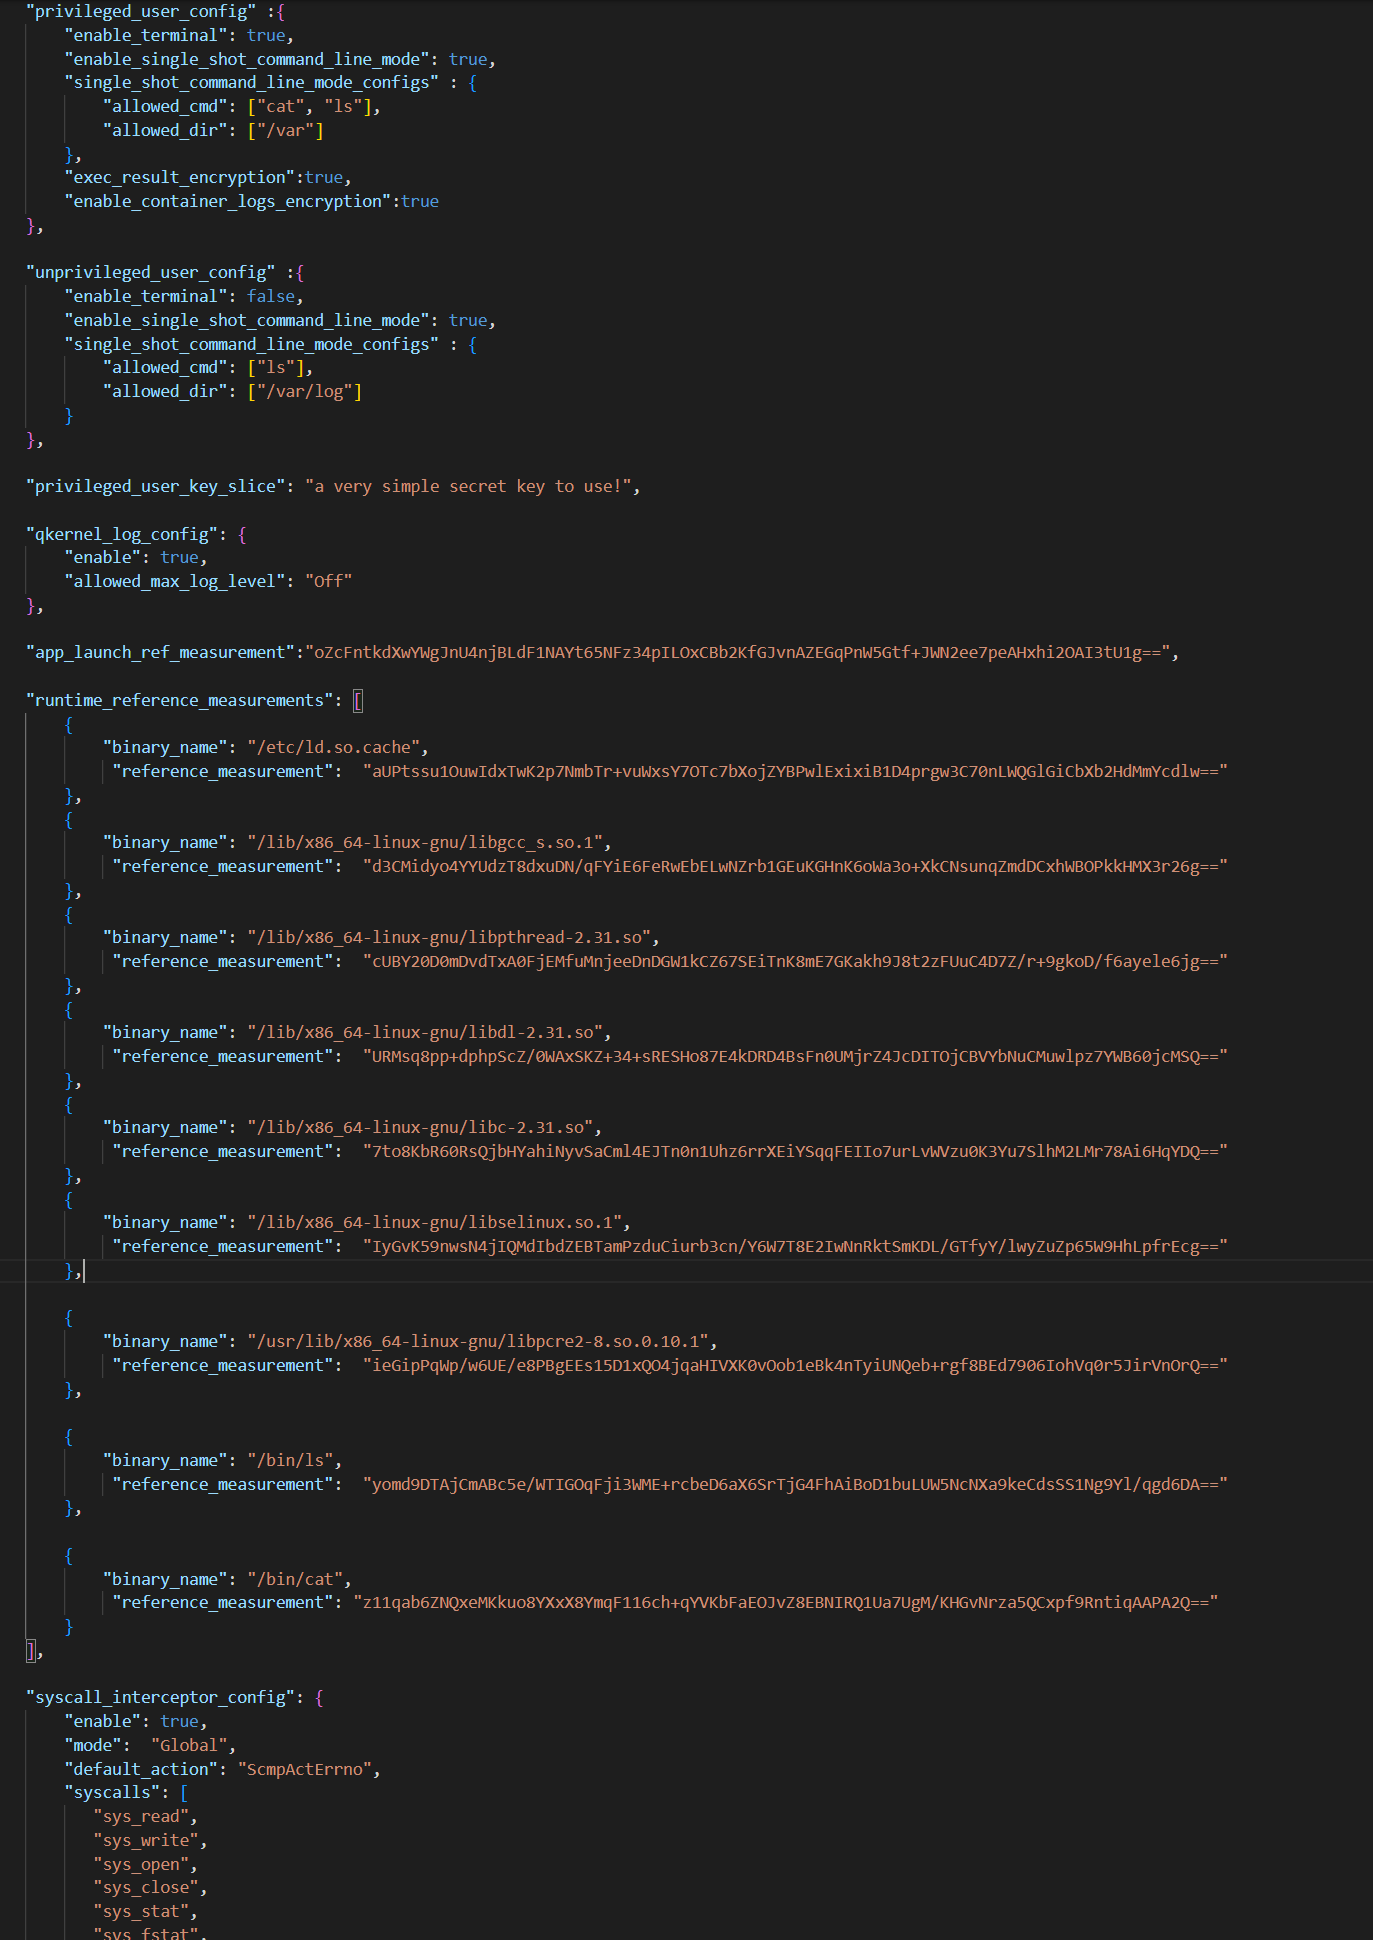
\includegraphics[width=0.9\linewidth]{images/generic_policy.PNG} 
      \caption{Enclave policy} 
      \label{fig:generic_policy} 
      \vspace{4ex}
    \end{subfigure}%% 
    \begin{subfigure}[b]{0.45\linewidth}
      \centering
      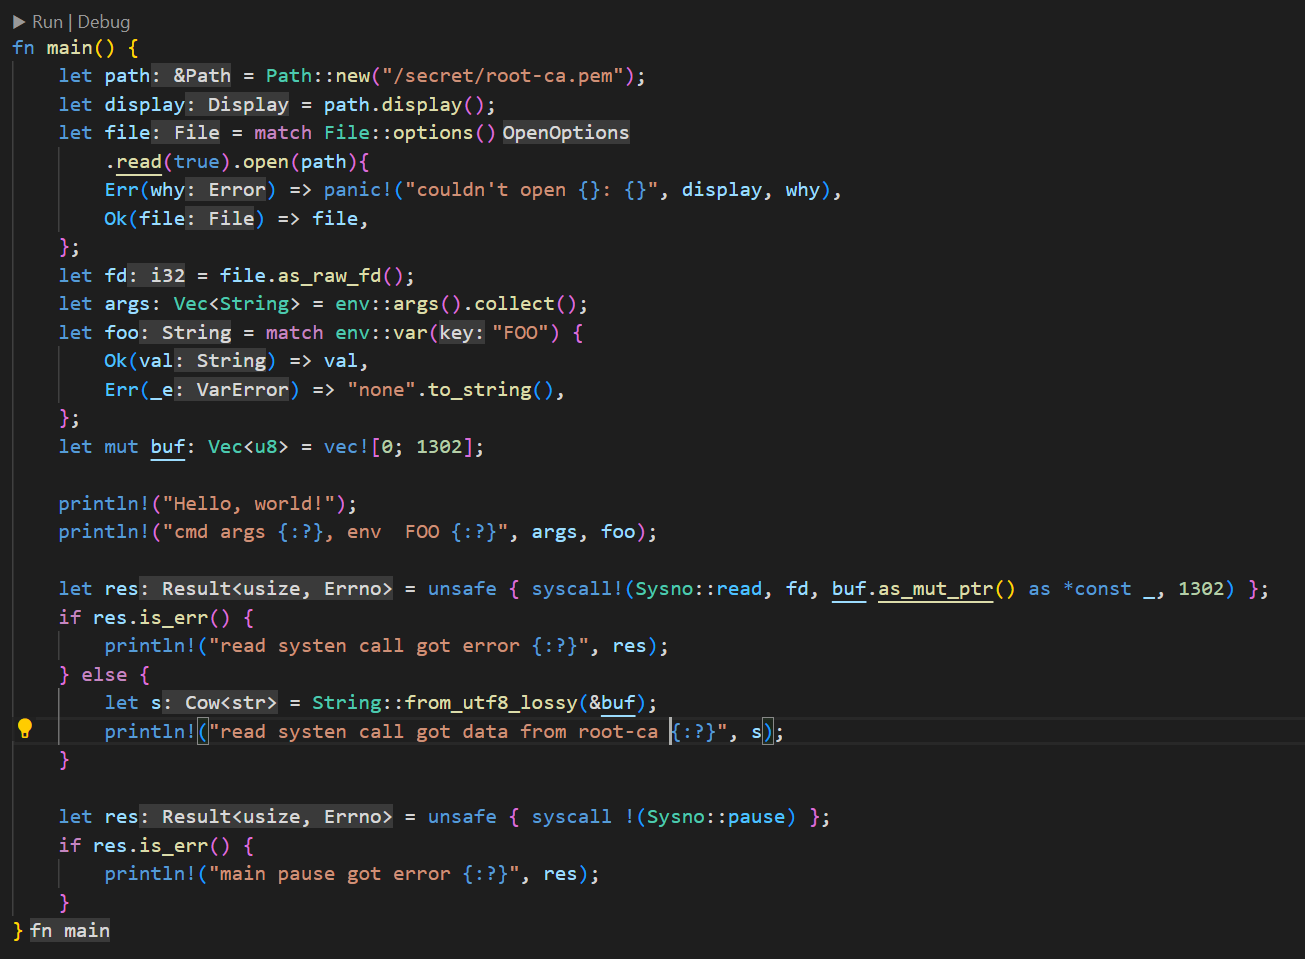
\includegraphics[width=0.9\linewidth]{images/analysis_workload.png} 
      \caption{Program used for the qualitative analysis} 
      \label{fig:analysis_workload} 
      \vspace{4ex}
    \end{subfigure} 
    \caption{Artifacts for demo in the qualitative analysis}
    \label{fig4} 
\end{figure}




This section outlines the configuration for the analysis. First, we set up the Confidential Quark and Vanilla Quark environments following the guidelines provided in the Quark demo repository~\cite*{Qaurk_Demo_for_qualitativ}. The policy used by Confidential Quark is shown in Figure~\ref{fig:generic_policy}. The policy specifies that the Enclave is in production mode. 
Privileged users can allocate terminals and issue cat and ls commands, while non-privileged level users can only issue ls commands. Privileged-level commands can be executed in the directory /var and its subdirectories, while non-privileged-level commands can only access the directory /var/log and its subdirectories. In addition, the Qlog manager is turned on. 
Since allowed\_max\_log\_level is set to OFF, Qkernel does not print any logs. Finally, the guest system call interceptor is activated and runs in ContextBase mode. The system call allowlist contains all system calls (0-451), some of which are not included in the figure due to space limitations.


Figure~\ref{fig:generic_policy} shows the example program used for the quantitative analysis. The program first print the environment variable and application parameter type secrets. It then accesses the secret "root-ca.pem" under directory /secret. The application-related secret is shown in Figure~\ref{fig5}. We use script~\cite*{secret_uploading_script} to deploy these secrets and the enclave 
policy to the secret manager. Note that the application is already containerized. The artifacts for the demo in the qualitative analysis and the YAML files for Deploying the demo can be found in commit~\cite*{artifacts_quarlitative}.

\begin{figure}[!htb] 
    \begin{subfigure}[b]{0.45\linewidth}
      \centering
      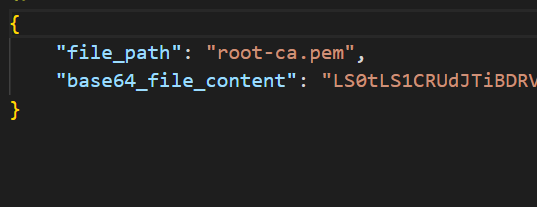
\includegraphics[width=0.9\linewidth]{images/file_secrets.PNG} 
      \caption{File type secrets} 
      \label{fig:file_secrets} 
      \vspace{4ex}
    \end{subfigure}%% 
    \begin{subfigure}[b]{0.45\linewidth}
      \centering
      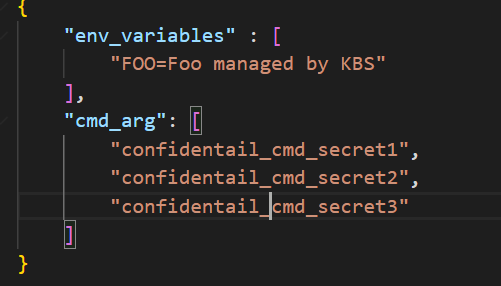
\includegraphics[width=0.9\linewidth]{images/cmd_env_secrets.png} 
      \caption{Args and Envv based secrets} 
      \label{fig:cmd_env_secrets} 
      \vspace{4ex}
    \end{subfigure} 
    \caption{Secrets for demo in the quantitative analysis}
    \label{fig5} 
\end{figure}


\subsection{Application secure Deployment}
\begin{figure}[!htb]
    \centering
    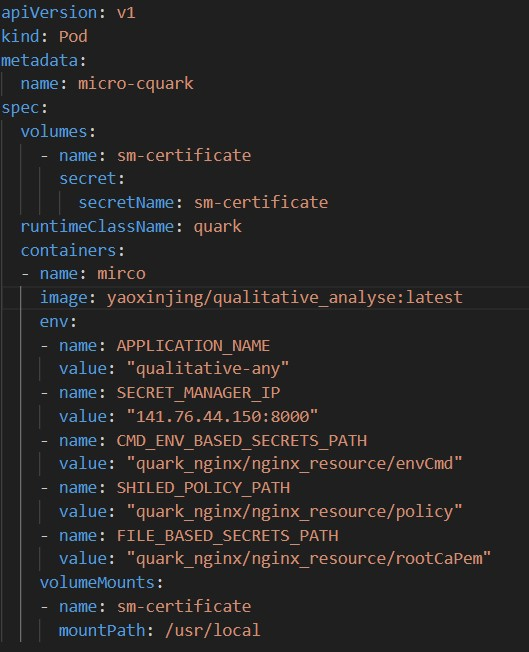
\includegraphics[height=0.3\textheight]{images/cquark_deploy_yaml.jpg}
    \caption[YAML for deploying an application in confidential Quark]{YAML for deploying an application in confidential Quark}
    \label{fig:cquark_deploy_yaml}
\end{figure}

Confidential Quark deploys the application using YAML, as shown in Figure~\ref{fig:cquark_deploy_yaml}. The new application deployment scheme and YAML are explained in Section~\ref{sec:secure_application_deployment}. Figure~\ref{fig:cquark_deployment} outlines the steps and outcomes of the application deployment process in the Confidential Quark environment.

Figure~\ref{fig:cquark_kbs_start} shows that the enclave successfully attests its identity to the secret manager during remote attestation and provisioning. Currently, the secret manager operates in native mode, verifying the consistency between the enclave start hash and the reference hash specified in the 
enclave owner's policy. The enclave's startup hash includes the measurement for application binaries, Qkernel configuration files, etc. (refer to Section III). As depicted in Figure~\ref{fig:cquark_deployment_result}, the enclave successfully retrieves the secret from the secret manager and prints them. It's worth 
noting that the directory named "secret" remains invisible from the host (as seen in Figure~\ref{fig:cquark_deployment_result_file_secret_mount_location}), as file type secrets and the filesystem mounted under the /secret directory are within the enclave。 Therefore, security issues~\ref{vulnerabilities:1},~\ref{vulnerabilities:7}, and~\ref{vulnerabilities:11} 
have been effectively resolved.


\begin{figure}[!htb]
    \subfloat[Secret manager succesfully autheticate enclave's state during remote attestation\label{fig:cquark_kbs_start}]{%
    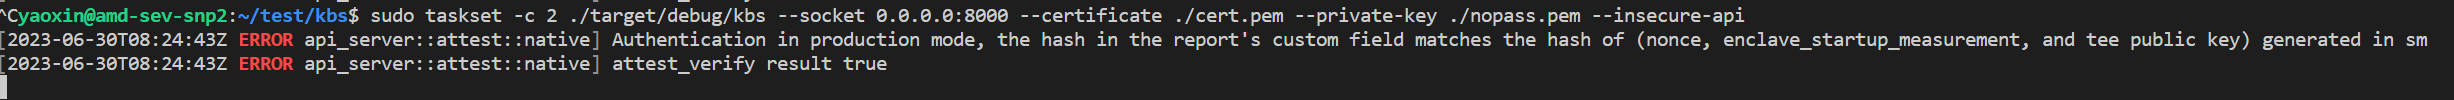
\includegraphics[clip,width=\columnwidth]{images/cquark_kbs_start.PNG}%
  }

    \subfloat[Application deployment process in confidential quark\label{fig:cquark_deployment_result}]{%
      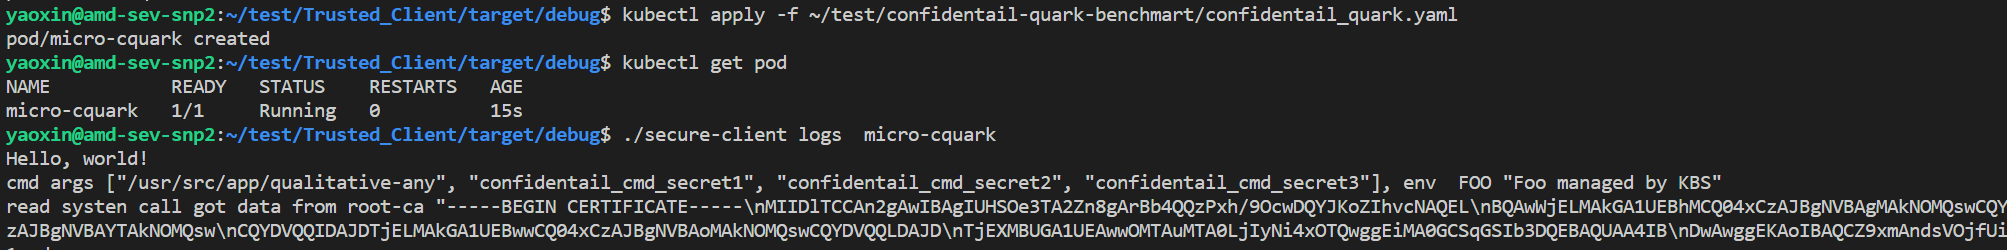
\includegraphics[clip,width=\columnwidth]{images/cquark_deployment_result.PNG}%
    }
    
    \subfloat[The way enclave manages the file type secrets\label{fig:cquark_deployment_result_file_secret_mount_location}]{%
      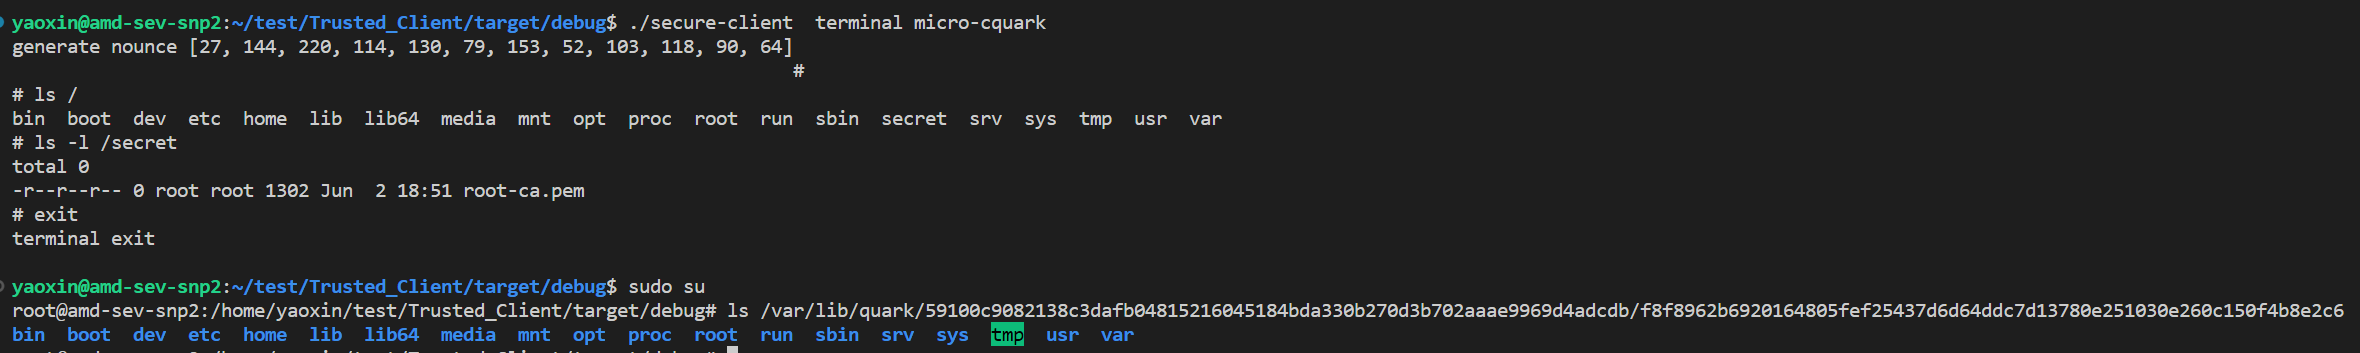
\includegraphics[clip,width=\columnwidth]{images/cquark_deployment_result_file_secret_mount_location.png}%
    }
    
    \caption[The result for application secure deployment in confidential Quark]{The result for application secure deployment in confidential Quark.\label{fig:cquark_deployment}}
\end{figure}





\subsection{Authentication and Access Control for EXEC Requests}


% \begin{figure}[H]

%     \subfloat[Accessing application log using securectl in confidential quark\label{fig:cquark_log_from_secure_ctl}]{%
%       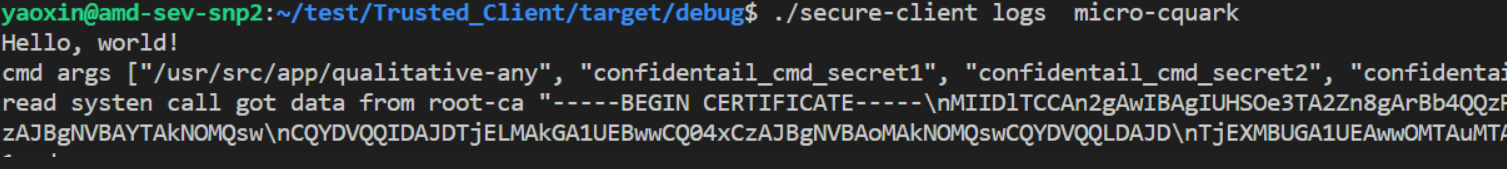
\includegraphics[clip,width=\columnwidth]{images/cquark_log_from_secure_ctl.png}%
%     }
    
%     \subfloat[Accessing application log using kubectl in confidential quark\label{fig:cquark_log_from_kubectl}]{%
%       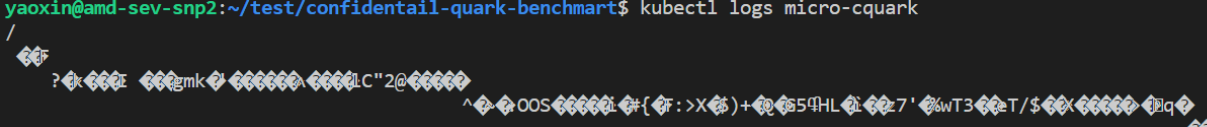
\includegraphics[clip,width=\columnwidth]{images/cquark_log_from_kubectl.png}%
%     }
    
%     \caption[Accessing application log through kubectl and securectl in confidential quark]{Accessing application log through kubectl and securectl in confidential quark. Figures 1 and 2 show that privileged users in cquark, i.e., 
%     application owners, have normal access to the application logs, while non\-privileged users using kubectl logs only obtain encrypted garbled code.}
% \end{figure}
\begin{figure}[!htb]

    \subfloat[The enclave rejects the privileged and non-privileged command ”ls /“"\label{fig:ls_exec}]{%
    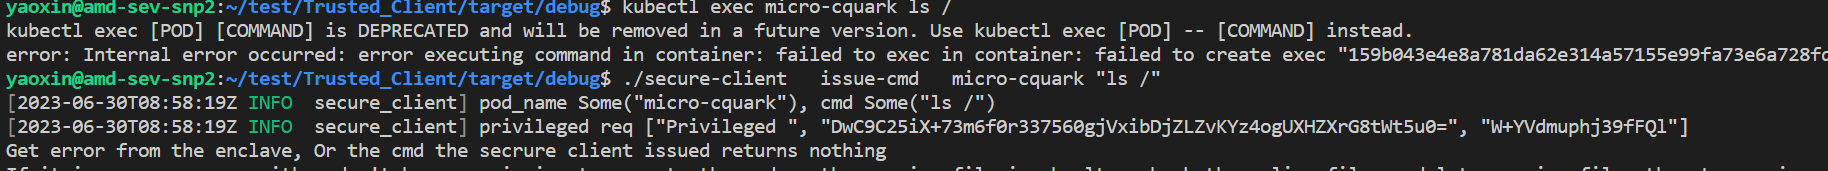
\includegraphics[clip,width=\columnwidth]{images/ls_exec.png}%
    }

    \subfloat[Issuing unprivileged command "ls /var/log"\label{fig:ls_allow_unprivileged}]{%
    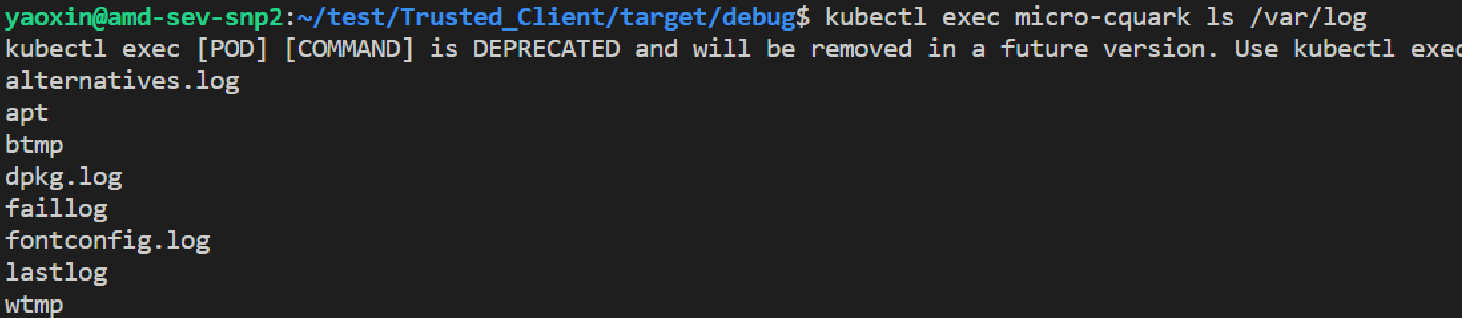
\includegraphics[clip,width=\columnwidth]{images/ls_allow_unprivileged.png}%
    }

    \subfloat[Issuing privileged command "ls /var/"\label{fig:ls_allow_previleged}]{%
      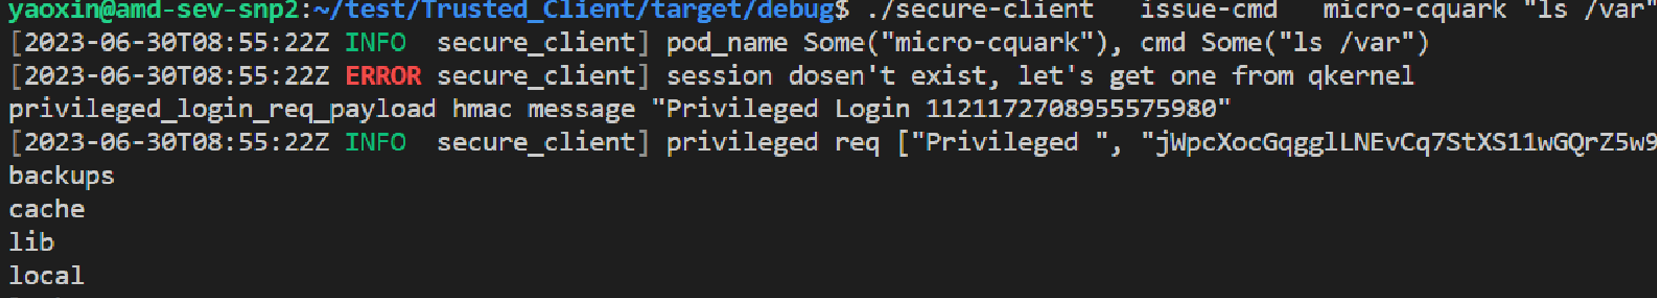
\includegraphics[clip,width=\columnwidth]{images/ls_allow_previleged.png}%
    }
    
    \subfloat[Issuing privileged command "cat" \label{fig:cat_pri}]{%
      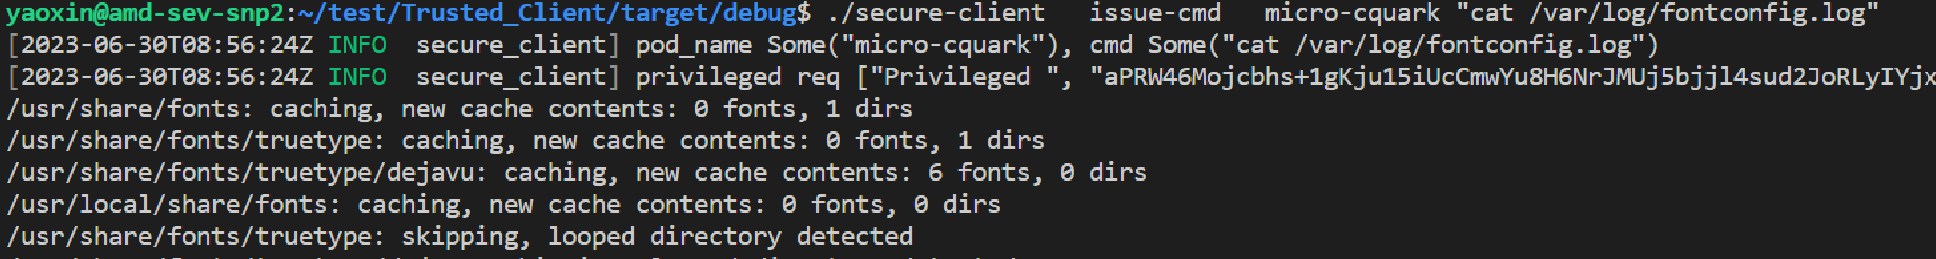
\includegraphics[clip,width=\columnwidth]{images/cat_pri.png}%
    }

    \subfloat[Issuing privileged command "cat" \label{fig:cat_unpri}]{%
    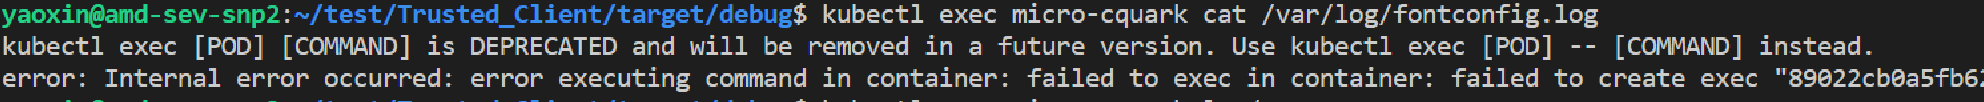
\includegraphics[clip,width=\columnwidth]{images/cat_unpri.png}%
  }

  \subfloat[Attempting to allocate a terminal through both securectl and kubectl\label{fig:cquark_terminal}]{%
  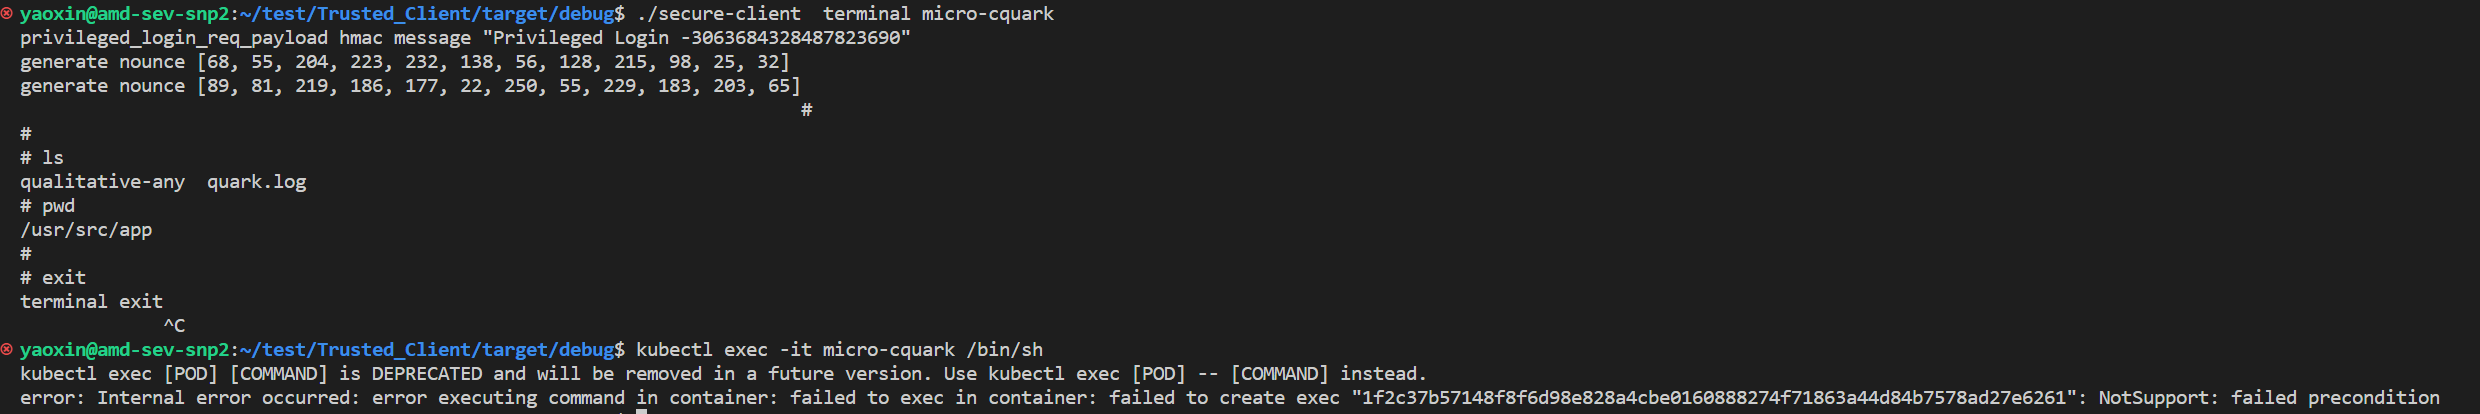
\includegraphics[clip,width=\columnwidth]{images/cquark_terminal.png}%
  }

  \subfloat[The privileged request is denied as the session is old\label{fig:seesion_is_old}]{%
  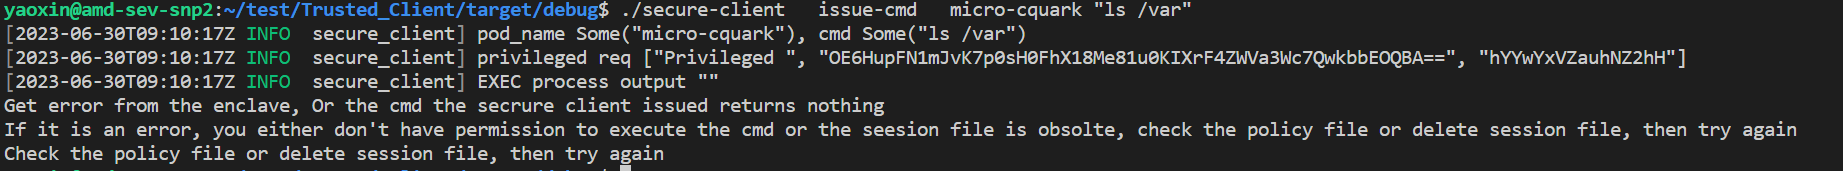
\includegraphics[clip,width=\columnwidth]{images/seesion_is_old.PNG}%
}
    
    \caption[The result of issuing  commands to enclave]{The result of issuing  commands to enclave\label{fig:exec}}
\end{figure}


In Section~\ref*{sec:design_EXEC_Requests}, we propose a novel schema for handling EXEC requests. As depicted in Figure~\ref{fig:ls_exec}, both privileged and unprivileged users are prohibited from executing the "ls /" command within the enclave due to the enclave policy's restriction on running commands in the root directory. 
Figure~\ref{fig:ls_allow_unprivileged} and~\ref{fig:ls_allow_previleged} illustrate that privileged and unprivileged users can issue the "ls /var" and "ls /var/log" commands to the enclave, respectively. This allowance stems from the enclave policy's command and directory allowlist, which 
includes these specific commands and their corresponding arguments. Conversely, since the command whitelist for non-privileged users excludes the "cat" command, unprivileged users are incapable of issuing the "cat" command to access the log file "/var/log/fontconfig.log."(figure~\ref{fig:cat_unpri}) 
Furthermore, as Figure~\ref{fig:cquark_terminal} shows, privileged users can spawn a terminal, while unprivileged users cannot. 
This is as expected since the unprivileged user's command allowlist does not include any terminal allocation instructions. 
Besides, securectl saves the session id and counter as a file locally. Securectl uses this file to build the frame structure for privileged commands. Compared to Figure~\ref{fig:ls_allow_previleged}, the same privilege command is denied in Figure~\ref{fig: seesion_is_old} as we modified the session 
id in the file. This shows that the enclave can prevent reply attacks from EXEC.


\begin{figure}[!htb]
    \centering
    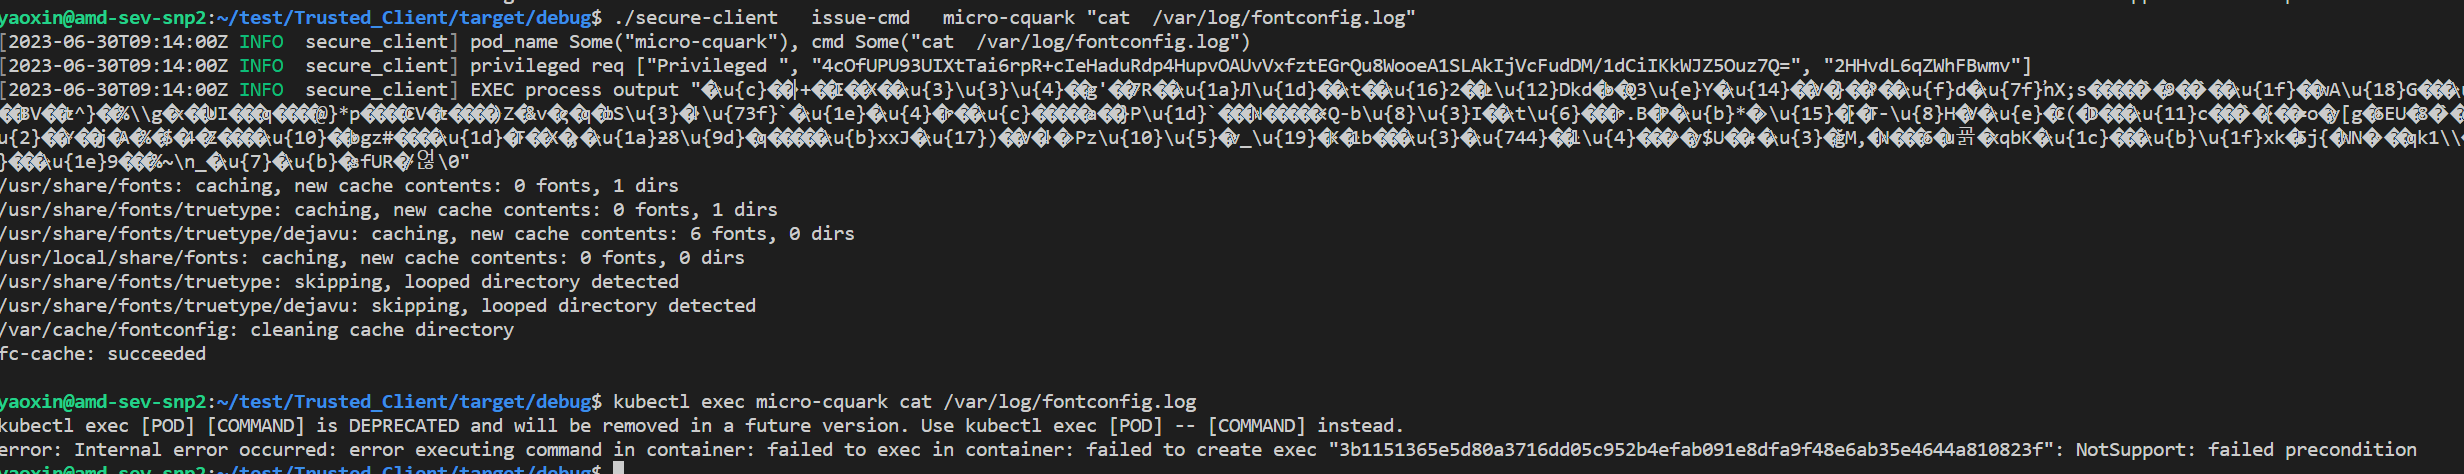
\includegraphics[width=1\textwidth]{images/cquark_priviled_cmd_result_protection.PNG}
    \caption[Process for securectl to handle privileged level commands]{Process for securectl to handle privileged level commands.}
    \label{fig:cquark_priviled_cmd_result_protection}
\end{figure}


In addition, we modified securectl to print the command it issues, and the execution result returned from the enclave. As shown in Figure~\ref{fig:cquark_priviled_cmd_result_protection}, both the EXEC command and its execution result are cryptographically protected. The protection mechanisms for the command and the execution result are 
discussed in Sections~\ref{sec:design_prptect_privileged_request} and~\ref{sec:design_STDIO_PROTECTION}, respectively.


This section shows that we can effectively address vulnerability~\ref{vulnerabilities:4} and ~\ref{vulnerabilities:6} identified in the security analysis.



\subsection{Guest User Space Process's STDIO Protection}
The application shown in Figure~\ref{fig:analysis_workload} is non-interactive. Since the no\_interactive\_process\_stdout\_err\_encryption option in the policy is true, the enclave will encrypt STDOUT and STDERR for privilege-level processes. Thus, only privileged users, namely the application owners, can view the logs using securectl (as shown in Figure~\ref{fig:cquark_log_from_secure_ctl}). On the other hand, non-privileged users who use the command 
"kubectl log" can only access the logs in ciphertext (as depicted in Figure~\ref{fig:cquark_log_from_kubectl}). Furthermore, Figure 4 showcases that the execution results of privilege-level commands are also encrypted.

\begin{figure}[!htb]

    \subfloat[Accessing application log using securectl\label{fig:cquark_log_from_secure_ctl}]{%
      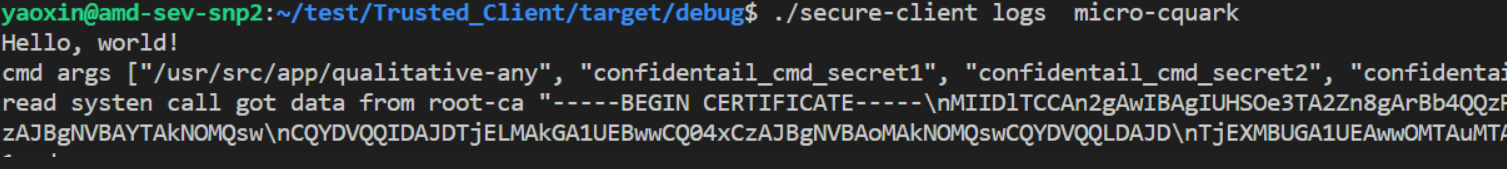
\includegraphics[clip,width=\columnwidth]{images/cquark_log_from_secure_ctl.png}%
    }
    
    \subfloat[Accessing application log using kubectl\label{fig:cquark_log_from_kubectl}]{%
      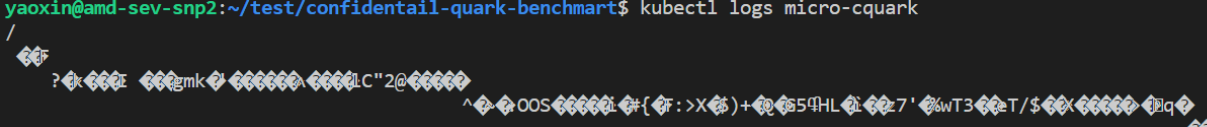
\includegraphics[clip,width=\columnwidth]{images/cquark_log_from_kubectl.png}%
    }
    
    \caption[Accessing non-interactive application log through kubectl and securectl]{Accessing non-interactive application log through kubectl and securectl}
\end{figure}

In the case of interactive applications, we use the busybox as an example. The corresponding YAML file for deployment can be found in commit~\cite*{artifacts_busybox}. Currently, the enclave lacks support for a terminal shielding layer. Nevertheless, we set the interactive\_porcess\_stdout\_err\_encryption option in the policy to true. 
This way, the enclave encrypts the STDOUT and STDERR outputs for the interactive application process. Figure~\ref{fig:attach_failed} illustrates the scenario where a non-privileged user can connect a terminal to the application. However, the terminal functionality is limited as the enclave only returns ciphertexts. 
Furthermore, the logs generated by the interactive application are also encrypted (Figure~\ref{fig:interactive_log}). These examples effectively showcase how our 
the proposed solution successfully mitigates vulnerabilities~\ref{vulnerabilities:5} and~\ref{vulnerabilities:3}.


\begin{figure}[!htb]

    \subfloat[Attaching to application using kubectl -it attach\label{fig:attach_failed}]{%
    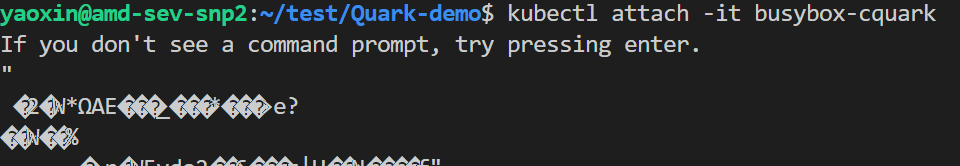
\includegraphics[clip,width=\columnwidth]{images/attach_failed.png}%
  }

  \subfloat[Accessing application log using kubectl\label{fig:interactive_log}]{%
  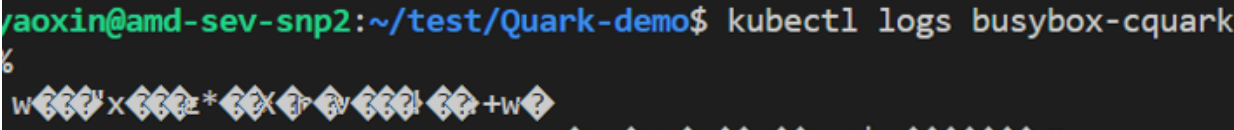
\includegraphics[clip,width=\columnwidth]{images/interactive_log.png}%
}
  
    \caption[Accessing logs and attaching to an interactive application ]{Accessing logs and attaching to an interactive application }
\end{figure}



\subsection{Qkernel Log Management}

In Vanilla Quark, the logs generated by Qvsivor and Qkernel are kept in the same file, /var/log/quark/quark.log. In order to differentiate the logs, we prefix the logs generated by Qkernel with the keyword "Qkernel" (refer to Figure~\ref{fig:vanilla_qkernel_Log}).
\begin{figure}[!htb]

    \subfloat[Vanilla Quark\label{fig:vanilla_qkernel_Log}]{%
    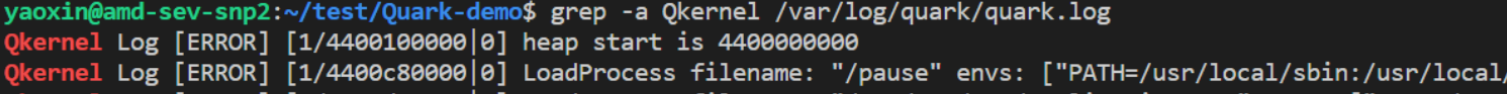
\includegraphics[clip,width=\columnwidth]{images/vanilla_qkernel_Log.png}%
  }

  \subfloat[Confidential Quark\label{fig:cquark_qkernel_log}]{%
  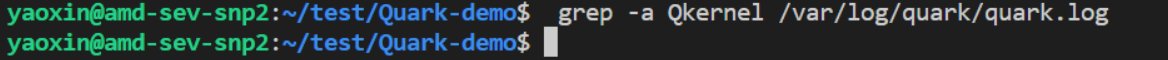
\includegraphics[clip,width=\columnwidth]{images/cquark_qkernel_log.png}%
}
  
    \caption[Accessing guest kernel log in confidential and vanilla Quark]{Accessing guest kernel log in confidential and vanilla Quark}
\end{figure}


In Confidential Quark, we set the Qlog manager's max log level to OFF. Therefore, the guest kernel logging system does not print logs to the host (Figure~\ref{fig:cquark_qkernel_log}).

\subsection{Qkernel Guest System Call Interception}

\begin{figure}[!htb]
    \centering
    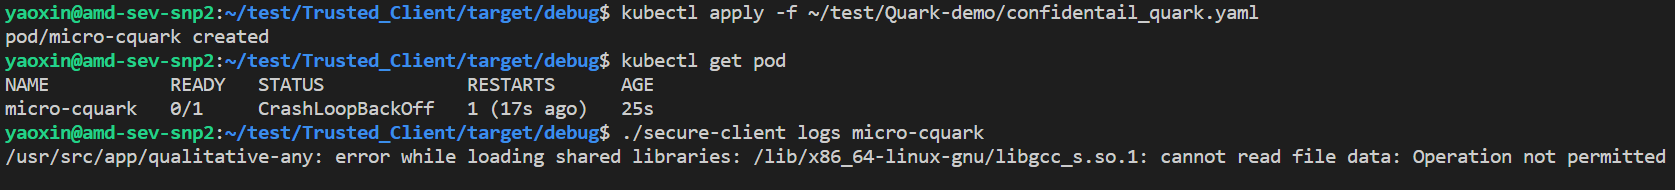
\includegraphics[width=1\textwidth]{images/application_failed_to_start_due_to_syscall_interceptor.png}
    \caption[Failed to run an application when the read system call is excluded from the system call interceptor's allowed list]{Failed to run an application when the read system call is excluded from the system call interceptor's allowed list}
    \label{fig:application_failed_to_start_due_to_syscall_interceptor}
\end{figure}


Figure ~\ref{fig:application_failed_to_start_due_to_syscall_interceptor} presents a demo of the guest interceptor. By revising the setting of the system interceptor in the enclave policy of Figure ~\ref{fig:generic_policy} to remove the read system call from the system call allowlist, 
the application process failed to start. The failure occurred because it lacked permission to execute the read system call for loading dynamic libraries.

\subsection{Application Runtime Measurements}




According to the discussion in Section~\ref{sec:Enclave_Runtime_Measurement}, the enclave measures the binaries loaded from the host at application runtime and compares the resulting hashes with the reference hashes in the enclave policy. Binary refers to shared libraries and executables. 

Figure~\ref{fig:cquark_runtime_runtime_lib_measurement_demo} shows a measurement demo of the runtime library. Regarding the setup, we intentionally reset the reference hash of the library "/lib/x86\_64-linux-gnu/libgcc\_s.so.1" in the enclave policy to empty and configure the maximum logging level of the Qlog manager to Info. Next, 
we deploy the policy to the secret manager and use the demo application in Figure~\ref{fig:analysis_workload}. The Qkernel logs in Figure~\ref{fig:cquark_runtime_runtime_lib_measurement_demo} show that the enclave encountered a crash due to a discrepancy between the measurements of the loaded library and the corresponding reference hash stored in the policy.


\begin{figure}[!htb]
    \centering
    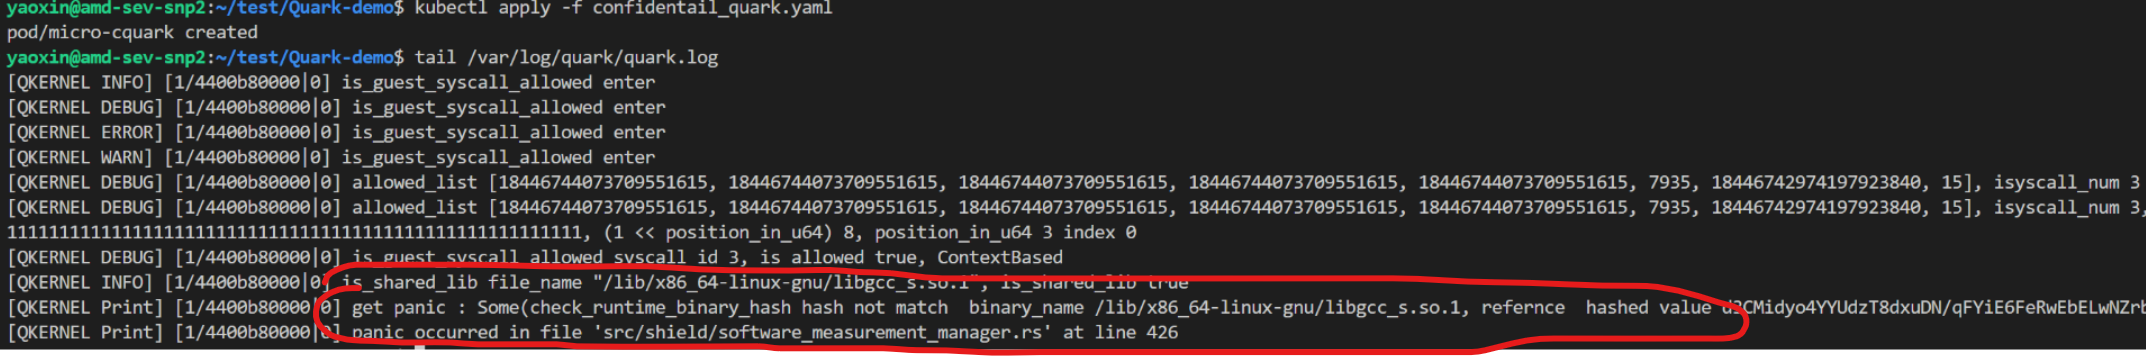
\includegraphics[width=1\textwidth]{images/cquark_runtime_runtime_lib_measurement_demo.png}
    \caption[Shared library measurement demo]{Shared library measurement demo}
    \label{fig:cquark_runtime_runtime_lib_measurement_demo}
\end{figure}




To demonstrate measuring the executable loaded during application runtime, we intentionally configured the enclave policy to set the reference hash for the "ls" binary to empty and the Qlog manager's max log level to Info. Then, we submit the new policy to the secret manager,  
redeploy the application, and issue the command "ls /var/log" to the enclave. Figure~\ref{fig:cquark_runtime_runtime_binary_measurement_demo}  shows that the command failed to get a response. By analyzing the Qkernel logs, we confirmed that the reason for the Qkernel crash was a mismatch between the reference hash of the ls binary and its actual hash.


\begin{figure}[!htb]
    \centering
    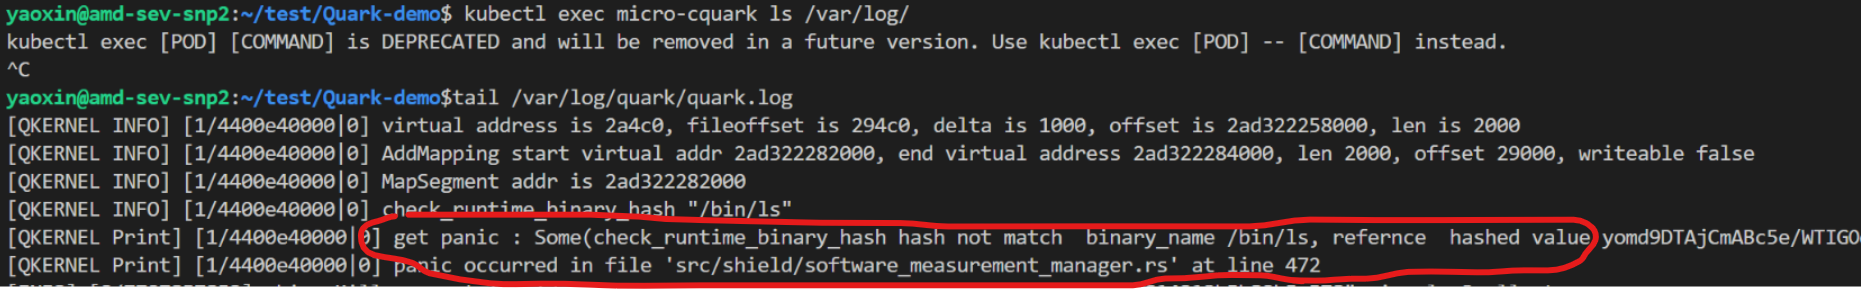
\includegraphics[width=1\textwidth]{images/cquark_runtime_runtime_binary_measurement_demo.png}
    \caption[Runtime binary measurement demo]{Runtime binary measurement demo}
    \label{fig:cquark_runtime_runtime_binary_measurement_demo}
\end{figure}



The above two examples highlight the ability of an enclave to refuse execution when an adversary tries to trick the enclave into loading harmful code during application runtime.

\subsection{Missing administration to application restartup}


As discussed in Section~\ref{sec:Enclave_Runtime_Measurement}, the enclave will measure the loaded binaries and shared libraries during the application rebuild process to extend the application restart hash. The enclave can ensure the rebuild process is correct by comparing the 
application startup reference hash to the restart hash.
\begin{figure}[!htb]

    \subfloat[Application restart workflow\label{fig:app_restart_eva}]{%
    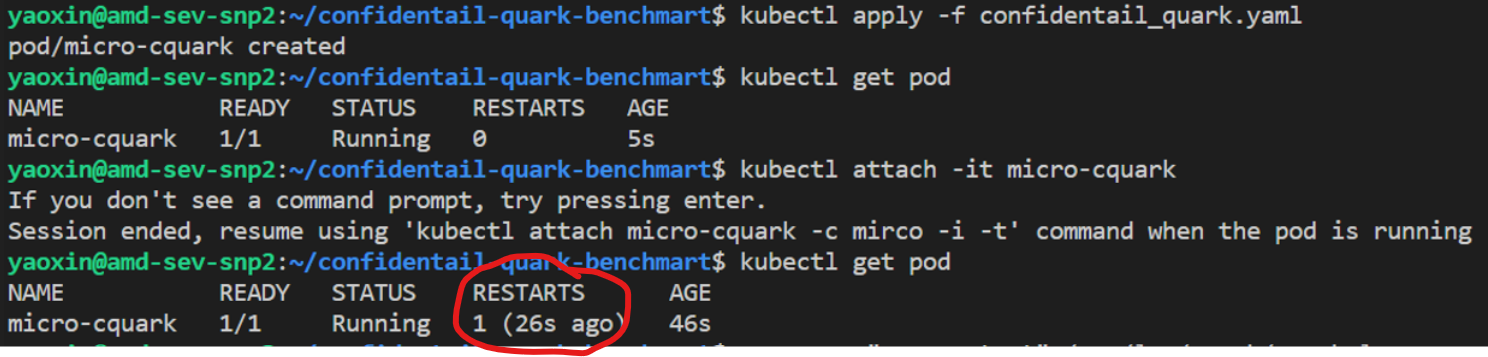
\includegraphics[clip,width=\columnwidth]{images/app_restart_eva.png}%
  }

  \subfloat[Qkernel log\label{fig:app_restart_result}]{%
  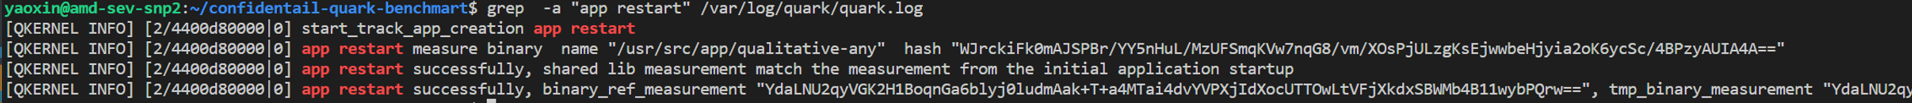
\includegraphics[clip,width=\columnwidth]{images/app_restart_result.png}%
}
  
    \caption[Demo for  administration to application restartup]{Demo for  administration to application restartup}
\end{figure}



The application restarting process is exemplified in Figure~\ref{fig:app_restart_eva}. In this example, we configure the Qlog manager’s max log level to ’Info’ in the enclave policy and add the keywords ’stdin: true’ and ’tty: true’ to the container spec of the YAML file used to deploy the 
application (Figure~\ref{fig:cquark_deployment}). These keywords keep the application’s stdin open and notify Kubernetes that it should be regarded as a terminal. We first create the application in the demo using the modified YAML file. Once the application starts, we use ’kubectl attach -it’ to 
attach to the application process and send ’ctrl c’ to the enclave. The ctrl c will cause the terminal IO redirection thread sends SIGINT to terminate the application, as discussed in section~\ref{sec:security_analyse_STDIO}. The output of the second ’kubectl get’ command confirmed that the application had successfully restarted. 

After analyzing the Qkernel log shown in Figure~\ref{fig:app_restart_result}, we found that Qkernel measured binaries and shared libraries loaded from the host during the application restart. The enclave compared the resulting measurements with the application startup reference hash to determine that the binaries and shared libraries loaded during the two startups were 
consistent.



% \begin{table}[H]
%     \tiny
%     \caption{Possible Vulnerability in upstream Quark in the context of Confidential Computing and suggested Solutions}
%     \label{crouch}
%     \begin{tabular}{  p{3.4cm}  p{3.4cm}  p{3.4cm} p{2cm} }
%         \toprule
% \textbf{Vulnerability}      
% & \textbf{Attack Example}   
% & \textbf{Possible Solution}
% & \textbf{Comment}  \\\midrule
% Physical Access Attacks
% & Offline DRAM Analysis          
% & Running the application in a secure virtual machine
% & Out of the scope   \\\hline
% Lack of protection to guest memory and register states          
% & Hypervisor reads private guest memory/cpu states                          
% & Running the application in a secure virtual machine
% & Out of the scope   \\\hline
% Paravirtualized filesystem sharing mechanism       
% & Hypervisor/Untrusted host process reads application’s credentials stored on host
% & Enable file system shielding layer to encrypt outbound and decrypt inbound data 
% & Out of the scope   \\\hline

% No security guarantee for communications over the Internet (unbounded network access to containers)     
% & Attacker access application’s credential by establishing a network connection to application using tools like, kubectl port-forward
% & Enable network shielding layer using TLS
% & Out of the scope   \\\hline

% Deploying Secrets via untrusted Entities (Kubelet, Containerd, Qvisor)    
% & File type secrets are mounted to container rootfs by qvisor, args and envv type secrets are passed to qkernel through qvisor
% & Offload the secrets deployment from qvisor by defining a new secure channel btw. relying party and guest kernel for secrets provisioning and storing secrets on guest memory
% & Problem solved  \\\hline

% Executing arbitrary command in container  
% & Attacker view application’s credentials stored on guest memory using kubectl exec cat command
% & Enable authentication and access control to kubectl exec in guest kernel
% & Problem solved  \\\hline


% Container log in plaintext managed by untrusted entity
% & Attacker reads application’s log message using kubectl logs container-name
% & Enable container STDOUT protection
% & Problem solved  \\\hline

% Storing Qkernel Log on host in plaintext
% & Cloud provider reads guest kernel’s log messages located in directory /var/log/quark
% & Enable qkernel log manager and set the log level to OFF
% & Problem solved  \\\hline

% Loading untrusted executable from host
% & Attackers may tamper with executables stored on the host and trick applications into executing compromised code to reveal secrets
% & Executable loaded into guest memory is measured and the results are send to relying party for executable integrity check
% & Problem solved  \\\hline

% Loading untrusted shared library from host
% & Attackers may tamper with shared libraries stored on the host and trick applications into executing compromised code to reveal secrets
% & Executable loaded into guest memory is measured and the results are send to relying party for executable integrity check
% & Problem solved  \\\hline

% Missing administration to application restart
% & Attacker may provide the guest with compromised executables, shared libraries, or wrong process spec when k8s requests the Qkernel to restart the crashed application
% & Compare the hash of the application rebuilding process with the hash of application's initial launching process stored on guest memory. If two hashes doesn’t match,  qkernel refuse the application restart request.
% & Problem solved  \\\hline


% No restriction to Container's syscalls (guest system calls)
% & Applications can be tricked into using vulnerable guest/host system calls, leading to disclosure of secrets
% & Using Guest system call interceptor to restrict the system calls application can use.
% & Problem solved  \\\hline


% Creating application process using untrusted process spec sent from host
% & Attacker may trick the qkernel into attaching a terminal to application process by modifying the "terminal" option in the process specification
% & Software measurement manager measure the loaded process specification and the results are send to relying party for integrity check
% & Problem solved  \\\hline


% Lack of runtime measurements
% & Secure VM like AMD SEV only calculate the hash of VM launching process, anything loaded to guest during runtime is not measured
% & Add software measurement manager to measure data loaded during runtime
% & Problem solved  \\\hline
% % objects and systems &
% % Underlying values       
% % & Plurality \\
%         \bottomrule
%     \end{tabular}
% \end{table}


\section{Quantitative Analysis}
In this section, we evaluate the performance of our system implementation in terms of both latency and throughput.

\subsection{Overview of Quantitative Analysis}

Our Benchmarking includes micro and macro-benchmarking. Microbenchmarks are performed to understand the latency overhead introduced by individual components in the shield, while macro benchmarks aim to evaluate the performance loss of running real-world applications in confidential Quark. 
The section is structured around the following subsections.

Section~\ref{Hardware_and_Software_Setup} first describes the hardware and software setup for benchmarking. Section~\ref{Attestation_Report_Syscall} then evaluates the speed of obtaining three types of attestation reports using a microbenchmark. We find that obtaining the simulation hardware report 
is 50\% slower than getting the other two software reports.

Subsequently, the overhead of the guest system call interceptor is evaluated in Section~\ref{bench_Interceptor}. The results show that the guest system interceptor imposes an overhead of 1.47x and 17x for guest-handled and host-handled system calls, respectively. Unlike vanilla Quark, 
confidential Quark stores file-type secrets on the guest's memory. Therefore, Section~\ref{bench_reading_file_secret} estimates the speed at which applications can access file-type secrets in vanilla Quark and confidentiality Quark. The results reveal that in confidential Quark, the speed of 
accessing file-type secrets is improved by a factor of 1.17.

Later, in Section~\ref{bench_issuing_Instructions}, we present latency benchmark results for issuing commands using kubectl in confidential and vanilla Quark. Compared to vanilla Quark, confidential Quark introduces 1.15 times overhead. Also, we compare the speed of sending the same commands in 
confidential Quark using kubectl and securectl. The results show that securectl executes 1.1 times faster than kubectl, even though the commands sent by securectl require additional cryptographic protection.

Then after estimating the performance of accessing binary-mapped memory regions, we observed that confidential Quark outperforms vanilla Quark in this regard (Section~\ref{accesiing_binary_mapped_memory}). Sequential access in confidential Quark is 1.86 times faster, while random reading and 
writing of binary-mapped memory regions exhibit approximately 1.08 times faster speed in confidential Quark. These results can be attributed to confidential Quark's measurement of binary files during program startup, which prompts the qkernel to load the files into memory, thus preventing 
page fault handling during runtime.

Section~\ref{micro_app_start_up} uses the "hello world" program to observe the effect of the number of file type secrets and the size of the measured binary on the application startup time duration. Findings indicate that the attestation and provisioning agent constitutes the bulk of the overhead 
when the size of the measurement data is less than 100 MB. Furthermore, when the number of file type secrets reaches 128, the overhead associated with the remote attestation and provisioning agent reaches 4500 ms, more than 70\% of the total program startup time.

In Section~\ref{macri_app_start_up}, we performed macro-benchmarks using Nginx~\cite*{nginx} and Redis~\cite*{redis}. Our benchmark explores the performance differences between applications running in confidential and vanilla Quark regarding startup time, exit time, and throughput. Our 
findings demonstrate that Redis and Nginx require 1.49X and 1.55X startup times in confidential Quark than in vanilla Quark, respectively. In terms of application exit time, Redis and Nginx exhibit almost the same performance when running in confidential and vanilla Quark. Furthermore, we utilize 
Redis-benchmark~\cite*{Redis_benchmark} and the Apache HTTP server benchmarking tool~\cite*{ab} to measure application throughput. The results indicate that Nginx and Redis running in confidential Quark encounter performance declines of approximately 9% and 20% due to guest system interceptor.

Section~\ref{tcb} analyzes the TCB overhead incurred by our implementation and compares the TCB sizes of Kata containers~\cite*{Kata-Containers} and confidential Quark. The results show that our implementation increases the binary of the quark guest kernel by about 1.47 times. Nevertheless, 
the TCB of confidential Quark is roughly one-sixteenth of the size of the Kata container.


% Further details, including the benchmark configuration and results can be found on page XX.

\subsection{Hardware and Software Setup}\label{Hardware_and_Software_Setup}

This section summarizes the hardware and software settings utilized for the benchmarks. Regarding hardware, all measurements are performed on a server with AMD EPYC 7443P 24-Core CPU and 4 DDR4-3200 Mhz-16GB RAM. Regarding software, the host OS is Ubuntu 20.04.6 LTS and Linux 5.19.0 kernel. 
Furthermore, the CPU governor is set to performance mode, and Hyper-Threading and Turbo Boost were disabled to establish a low-noise environment for benchmarking with reproducible results. Besides, all test binaries, namely Qvisor, Qkernel, and the ”hello-world” program in List~\ref{code1}, are built in 
release mode. Unless otherwise mentioned, the vanilla Quark is in version v0.2.0, and confidential Quarkuses use this commit~\cite*{qualitativ_confidentail_quark}.


Regarding the tools for measuring latency, since all benchmark objects are located in the guest, we use the guest system call clock\_gettime(monotonic)~\cite*{clock_gettime} for time measurement and print the results to the host using the Qkernel logging system. The 
benchmarking framework~\cite*{benchamark_framework} can analyze the results by parsing the Quark log under the host directory /var/log/Quark. In addition, all benchmarks are performed multiple times. The following sections illustrate the measurement results in average time and variance format.



\subsection{Micro-benchmark – Attestation Report Syscall}\label{Attestation_Report_Syscall}

Confidential Quark enables applications to obtain three types of attestation reports via a system call. The type of the report includes simulated AMD SEV SNP report, software reports signed by KBS key, or software reports signed by the application. This section assesses the speed with which the 
application acquires various reports. For this purpose, we prepared a Rust microbenchmark\cite*{benchamark_Attestation_Report_Syscall}. In order to ensure stable results, the test program submitted 10,000 requests for each type of report to the Qkernel. The benchmark program is containerized, 
and the YAML file for the deployment can be found in the repository~\cite*{perf_test_repo}.

\begin{figure}[!htb]
    \centering
    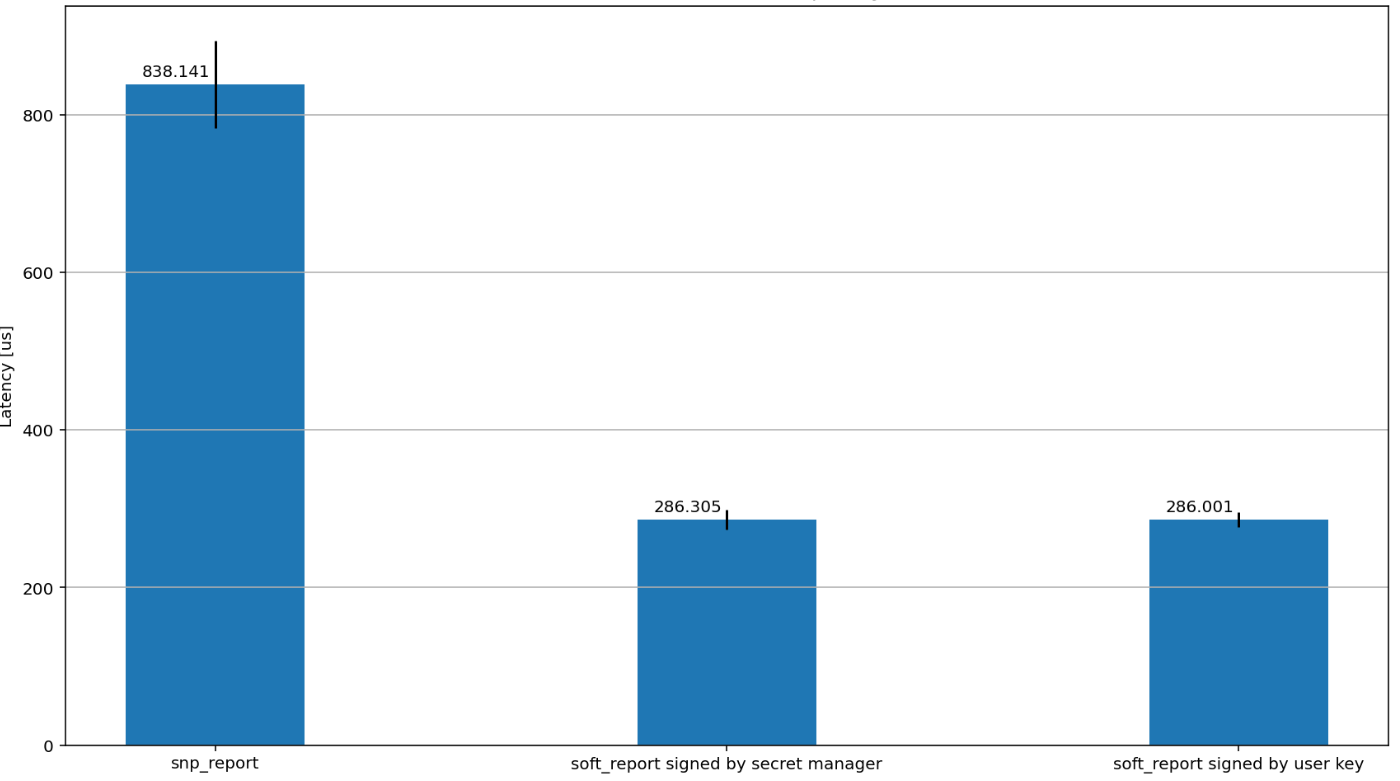
\includegraphics[width=0.5\textwidth]{images/perf_attestation_report_result.PNG}
    \caption[Benchmark result of Attestation Report Syscall]{Qkernel Attestation Report Syscall Benchmark Result}
    \label{fig:perf_attestation_report_result}
\end{figure}

Figure~\ref{fig:perf_attestation_report_result}  depicts the result. The data reveal that requesting a simulated hardware report takes approximately 838.141us, whereas acquiring the two software reports needs only about 286us. This difference stems from the fact that generating the hardware report involves expensive operations 
such as virtual machine exit, loading dummy SNP report from the disk, etc. Consequently, obtaining a simulated hardware report is significantly slower than a software report.


\subsection{Micro-benchmark – Qkernel Syscall Interceptor}\label{bench_Interceptor}

We prepare a micro-benchmark to investigate the latency overhead introduced by intercepting guest system calls~\cite*{benchamark_systemcall_intercetion}. The benchmark executes a selected system call 100,000 times and outputs the average and variance time. The YAML file for deploying this benchmark is 
in repository~\cite*{perf_test_repo}. The benchmark test four system calls: getpid, getppid, read, and write. Since Qkernel already implements process and thread objects, calling getpid or getppid using syscall instruction prompts Qkernel to directly return the corresponding pid/ppid without interference from the host. This provides us with a clear 
understanding of the overhead introduced by the interceptor. Additionally, we measured the execution time of read() and write() system calls for confidential and vanilla Quark to evaluate the overhead that the interceptor brought to the host-handled system calls.

\begin{figure}[!htb]
    \centering
    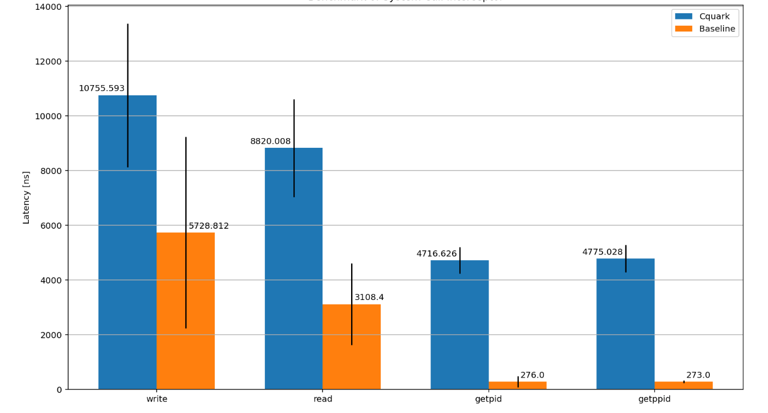
\includegraphics[width=0.5\textwidth]{images/ben_results_syscall_interceptor.PNG}
    \caption[Benchmark result of Syscall Interceptor]{Latency comparison of executing system calls in confidential VS vanilla Quark. The latency is thereby measured using the guest system call clock\_gettime(monotonic). 
        Each system call is executed 100,000  times in a tight loop. Read and write buffer size is 100 bytes}
    \label{fig:ben_results_syscall_interceptor}
\end{figure}

The test results in Figure~\ref{fig:ben_results_syscall_interceptor} reveal that vanilla Quark takes only around 270 ns to execute a single getpid and getppid call, while confidential Quark takes approximately 4716 ns. This indicates that the guest system call interceptor causes a delay of about 4500 ns per system call. Moreover, a 
comparable latency overhead is introduced for read and write system calls, i.e.,4500 ns. However, read and write system calls are processed on the host side and take longer. Thus their processing time in confidential Quark rises less significantly than that of getpid and getppid. To summarize, in 
confidential Quark, host-handled system calls (i.e., write and read) and guest-handled-only (e.g., getpid and getppid) are 1.47x and 17x slower, respectively, compared to vanilla Quark。 The interested reader is referred to Section~\ref*{sec:impl_interceptor} for information on the system call 
interceptor overhead sources.

\subsection{Micro-benchmark – Speed of Reading file base secret}\label{bench_reading_file_secret}

Compared to vanilla Quark, confidential Quark stores file-type secrets on guest memory. Hence, this benchmark~\cite*{benchamark_filebase_secret}  aims to evaluate the performance enhancement achieved from accessing file type secrets in confidential Quark. 
The benchmark measures the total time to perform one open() and read() operation on a file type secret in confidential and vanilla Quark. The file size is 1302 bytes. The test performs 10,000 open and read operations, and the read buffer size is 100 bytes. The YAML file used to deploy this test 
is in repository~\cite*{perf_test_repo}.

\begin{figure}[!htb]
    \centering
    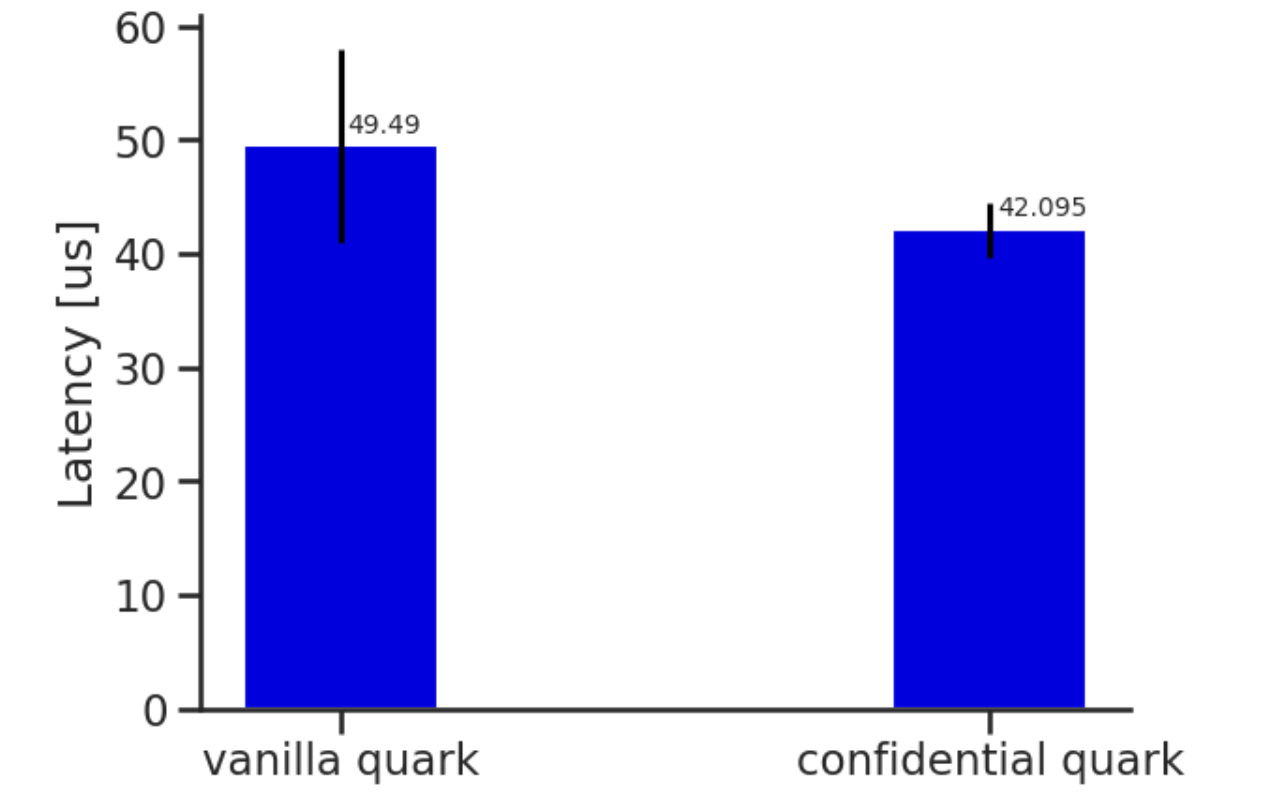
\includegraphics[width=0.5\textwidth]{images/reading_speed_of_file_type_secrets_in_Baseline_and_Cquark.PNG}
    \caption[Speed test for accessing file type secrets in Confidential Quark and Normal Quark]{Speed test for accessing file type secrets in Confidential Quark and Normal Quark.}
    \label{fig:reading_speed_of_file_type_secrets_in_Baseline_and_Cquark}
\end{figure}

The results shown in Figure~\ref{fig:reading_speed_of_file_type_secrets_in_Baseline_and_Cquark} reveal that confidential Quark's performance in accessing file-type secrets is competitive with vanilla Quark. Surprisingly, the speed in 
confidential Quark is only 1.17 times better. The likely reason for this is that the overhead of the guest system call interceptor in confidential Quark partially offsets the overhead incurred by the VM exit in vanilla Quark.

\subsection{Micro-benchmark – Latency Test for issuing Instructions to Application}\label{bench_issuing_Instructions}

This section presents the results of tests conducted to assess the latency of issuing instructions to applications in confidential Quark. The tests involved comparing the latency of sending commands using kubectl in confidential and vanilla Quark and the speed comparison test for issuing 
unprivileged and privileged commands in confidential Quark using kubectl and securectl, respectively. As such, the test framework is extended to issue specific instructions to an application using either kubectl or securectl while recording command execution time~\cite*{benchamark_perf_kubectl}. 
Besides, each command is issued 1,000 times to ensure dependable results. Due to time constraints, we chose four commonly used commands for the following testing: pwd, ls, cat, and cp.



\begin{figure}[!htb] 
    \begin{subfigure}[b]{0.5\linewidth}
      \centering
      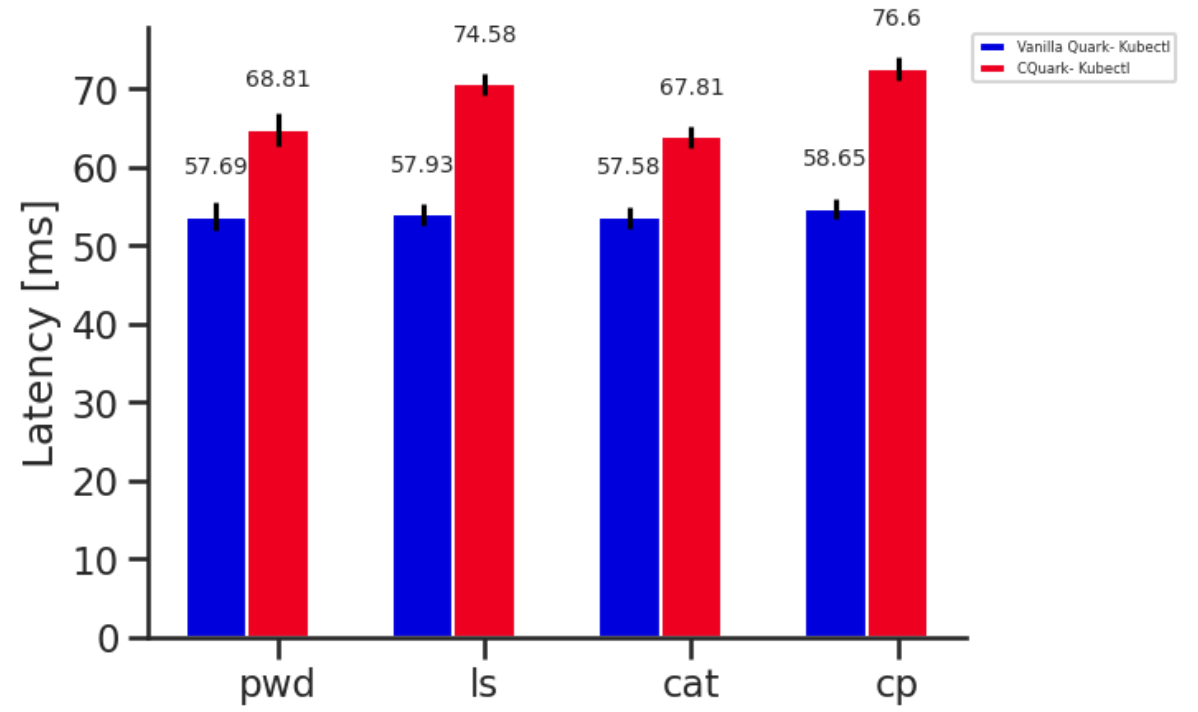
\includegraphics[width=1\textwidth]{images/speed_of_issuing_cmd_in_cquark_upstream_quark.PNG} % first figure itself
      \caption{Issueing commands}
      \label{fig:speed_of_issuing_cmd_in_cquark_upstream_quark}
      \vspace{4ex}
    \end{subfigure}%% 
    \begin{subfigure}[b]{0.5\linewidth}
      \centering
      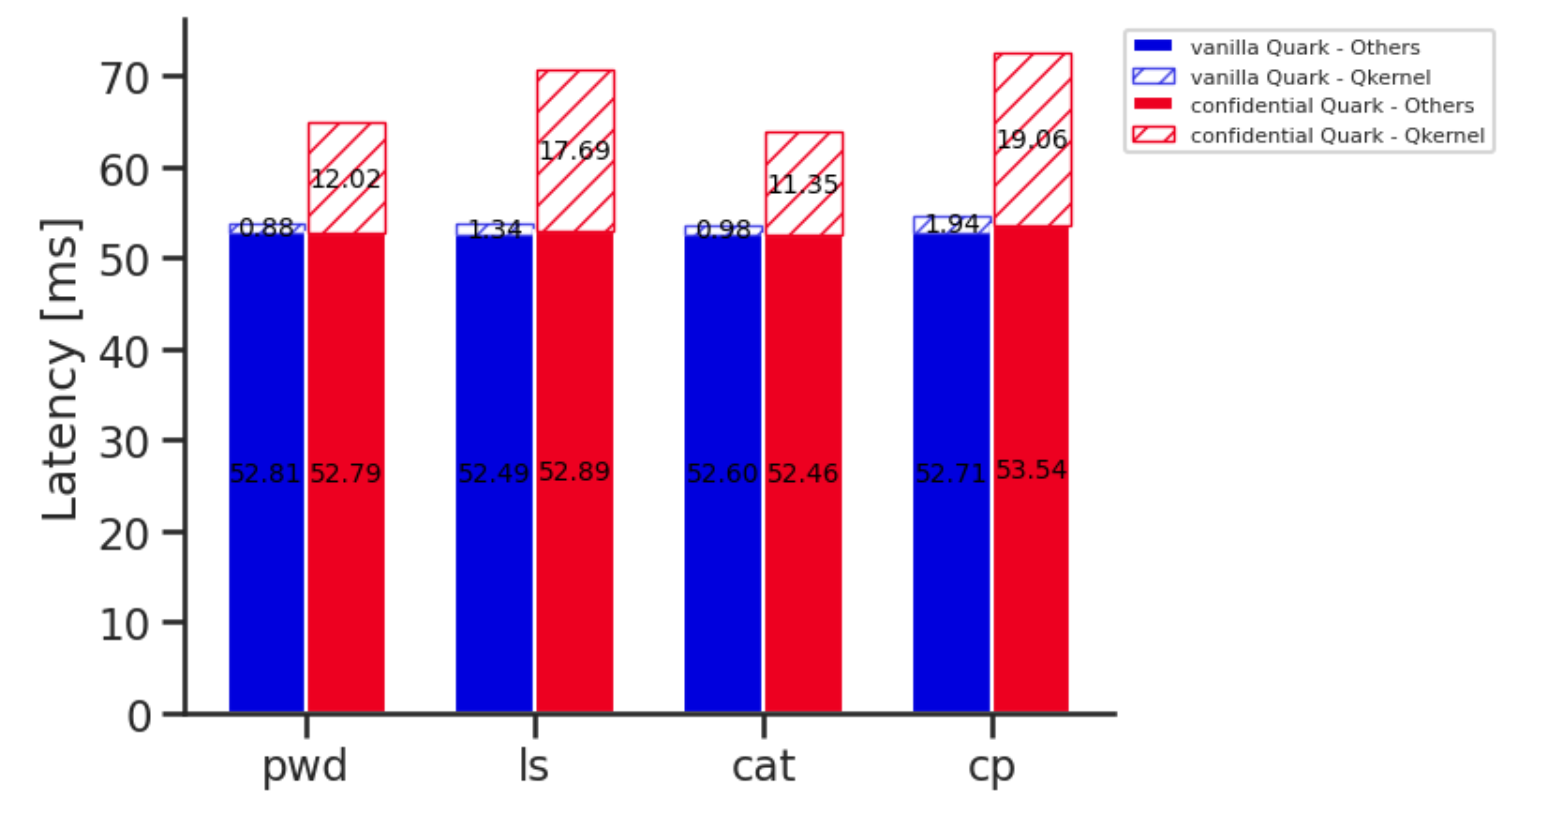
\includegraphics[width=1\textwidth]{images/timeshare_issuing_cmd_in_cquark_upstream_quark_kubectl.png} % second figure itself
        \caption{Percentage of time that Qkernel and others take to execute a command}
        \label{fig:timeshare_issuing_cmd_in_cquark_upstream_quark_kubectl}
      \vspace{4ex}
    \end{subfigure} 
    \caption{Latency comparison of issuing instruction in confidential vs vanilla Quark}
    \label{fig8} 
\end{figure}


The results in Figure~\ref{fig:speed_of_issuing_cmd_in_cquark_upstream_quark} illustrate issuing instructions using Kubectl in confidential Quark is more expensive than in vanilla Quark. Figure~\ref{fig:timeshare_issuing_cmd_in_cquark_upstream_quark_kubectl} exhibits that the additional overhead in confidential Quark comes from the Qkernel since it needs to authenticate and access control for each 
command and measures the command binary. Besides, the guest system interceptor also places an extra burden on Qkernel to execute commands.



\begin{figure}[!htb] 
    \begin{subfigure}[b]{0.5\linewidth}
      \centering
      \centering
      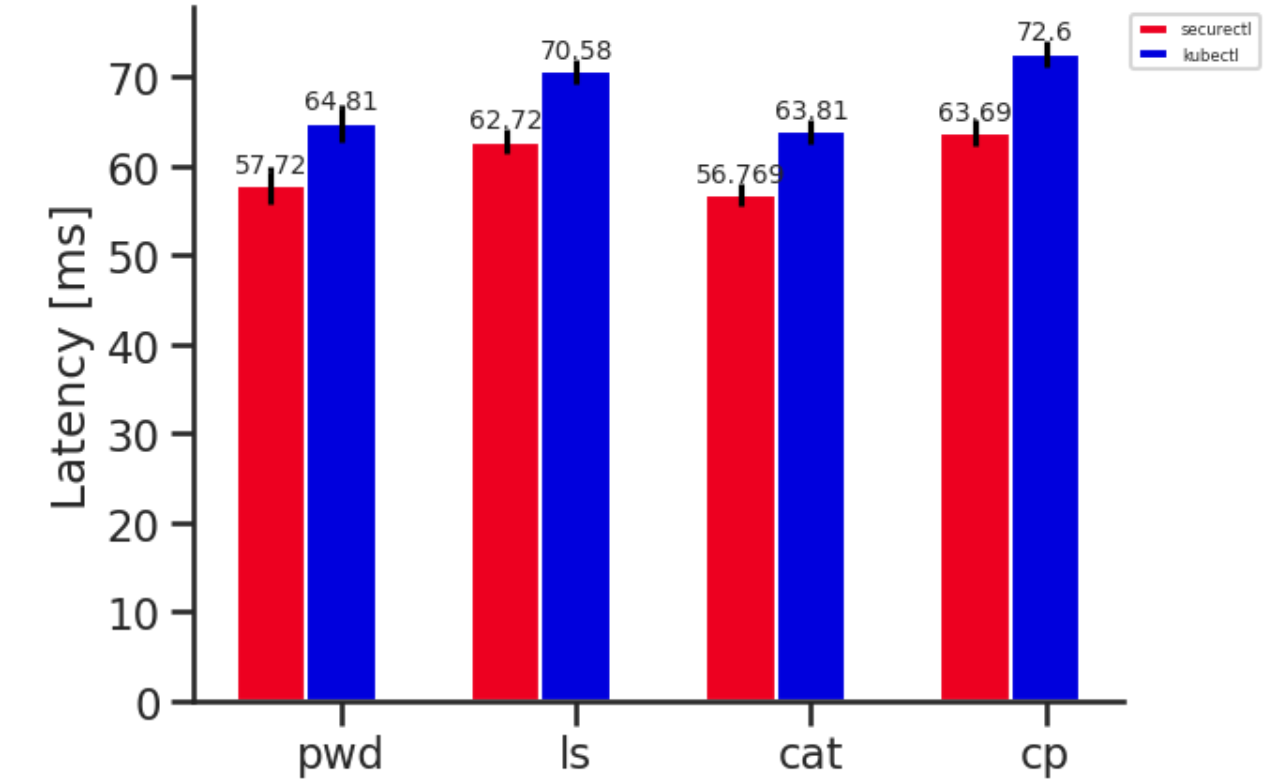
\includegraphics[width=1\textwidth]{images/speed_of_issuing_cmd_in_cquark_kubctl_securectl.png} % first figure itself
      \caption{Issueing commands}
      \label{fig:speed_of_issuing_cmd_in_cquark_kubctl_securectl}
      \vspace{4ex}
    \end{subfigure}%% 
    \begin{subfigure}[b]{0.5\linewidth}
      \centering
      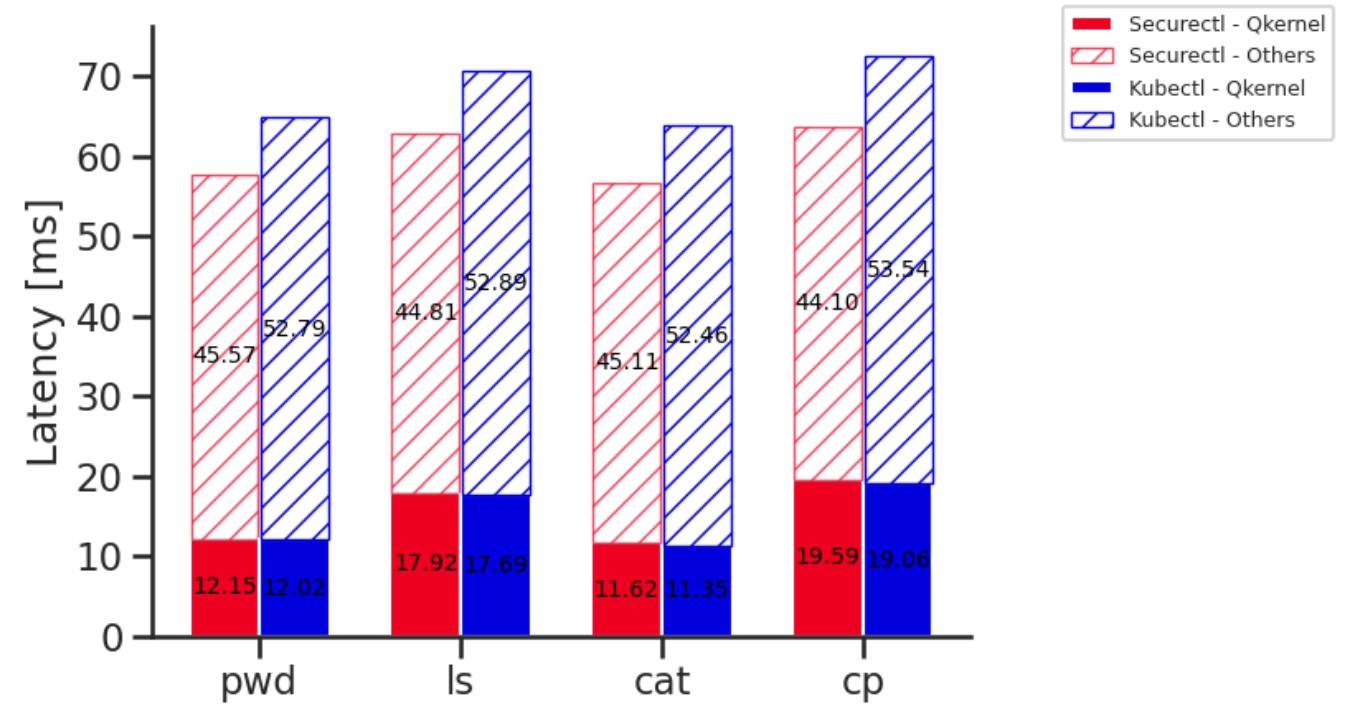
\includegraphics[width=1\textwidth]{images/timeshare_issuing_cmd_in_cquark_kubectl_securectl.png} % second figure itself
      \caption{Percentage of time that Qkernel and others take to execute a command}
      \label{fig:timeshare_issuing_cmd_in_cquark_kubectl_securectl}
      \vspace{4ex}
    \end{subfigure} 
    \caption{Latency comparison of issuing privileged vs. unprivileged instruction in confidential Quark}
    \label{fig9} 
\end{figure}



Figure~\ref{fig:speed_of_issuing_cmd_in_cquark_kubctl_securectl} compares the time required to issue privileged and unprivileged commands using Securectl and Kubectl in confidential Quark. The results show that issuing privileged commands is much faster than issuing unprivileged commands. 
This finding is counterintuitive since privileged instructions require additional cryptographic protection, which implies executing additional code. To investigate this further, we measured the percentage of time that Qkernel and other components take to execute a command. The other components 
refer to the tools for issuing instructions, i.e., kubectl or securectl, the Kubernetes components used to transfer commands. The results in Figure~\ref{fig:timeshare_issuing_cmd_in_cquark_kubectl_securectl} show that Qkernel takes roughly one millisecond longer to execute privileged commands than it does to execute unprivileged commands. However, non-privileged level commands spend significantly more 
time in the other components than privileged commands (dashed-filled boxes). The only difference between the other components for the privileged and unprivileged commands is the tool used to issue the instructions. This means that securectl is more lightweight than 
kubectl and thus offsets the cryptographic protection overhead of privileged commands.







% \begin{figure}[H]
%     \centering
%     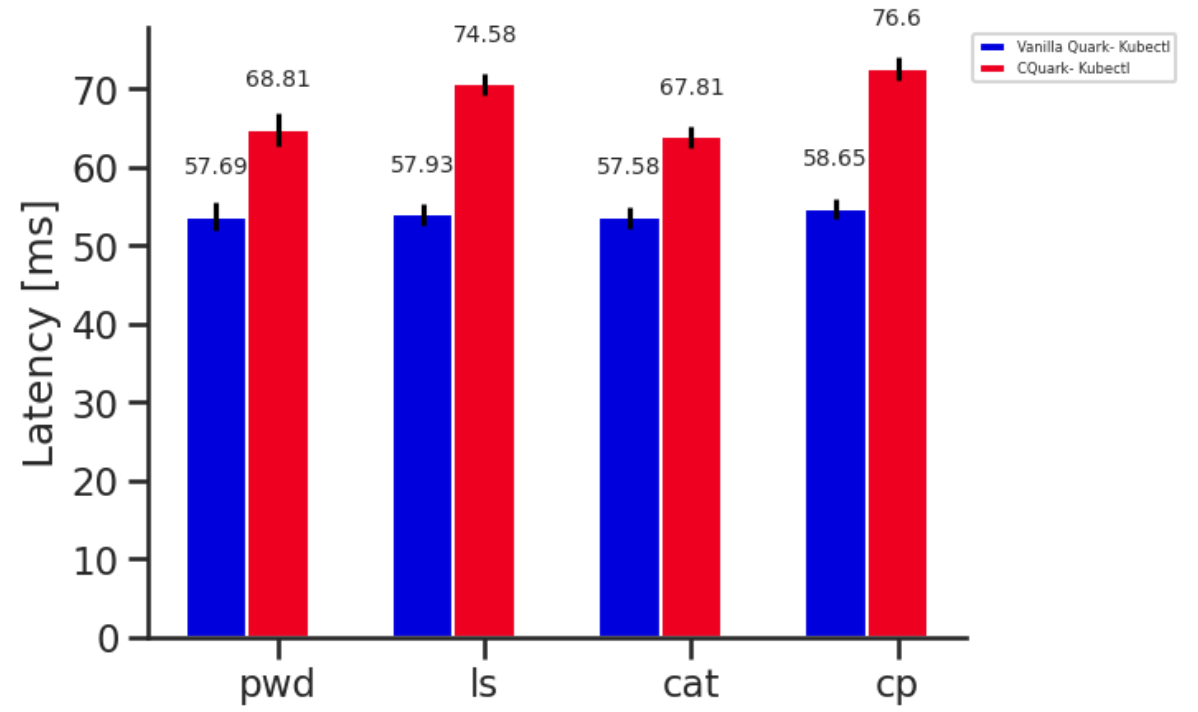
\includegraphics[width=0.8\textwidth]{images/speed_of_issuing_cmd_in_cquark_upstream_quark.PNG}
%     \caption[Benchmark result - Latency Comparison of sending Commands to Application in Cquark vs vanilla Quark]{A latency comparison test of sending commands to applications in cquark vs vanilla quark.  The test selects four 
%     commonly used Linux commands as samples, each being executed one thousand times. The results indicate that utilizing Kubectl exec to issue instructions to applications in cquark takes over 9\% longer than in vanilla quark.
%     }
%     \label{fig:speed_of_issuing_cmd_in_cquark_upstream_quark}
% \end{figure}




% \begin{figure}[H]
%     \centering
%     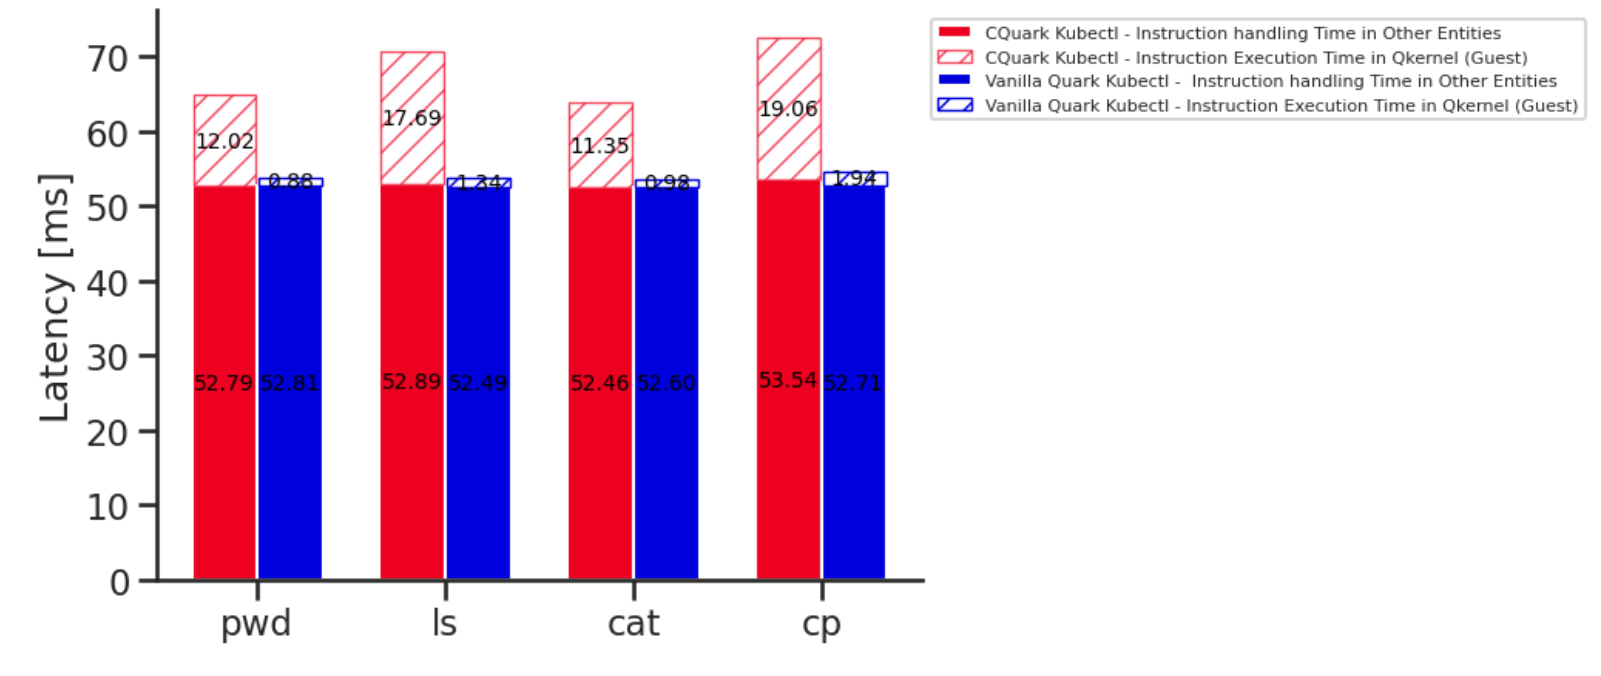
\includegraphics[width=0.8\textwidth]{images/timeshare_issuing_cmd_in_cquark_upstream_quark_kubectl.PNG}
%     \caption[Benchmark result - The processing time for each component during the instruction execution lifecycle in confidential vs in vanilla Quark]{Benchmark result of evaluating the percentage of time spent by each component in processing instructions during the instruction execution lifecycle 
%     in confidential vs in vanilla Quark . Here the components refer to kubectl,  Kubernetes components for instructions transmission, like containerd, etc., and Qkernel for instruction execution. 
%     Each bar in the figure represents the total execution time of an instruction whereby the color-filled section represents the time qkernel used for instruction execution, while the dashed-filled segment implies the time other components took for instruction issuing, transmission, and result handling.
%     }
%     \label{fig:timeshare_issuing_cmd_in_cquark_upstream_quark_kubectl}
% \end{figure}



% \begin{figure}[H]
%     \centering
%     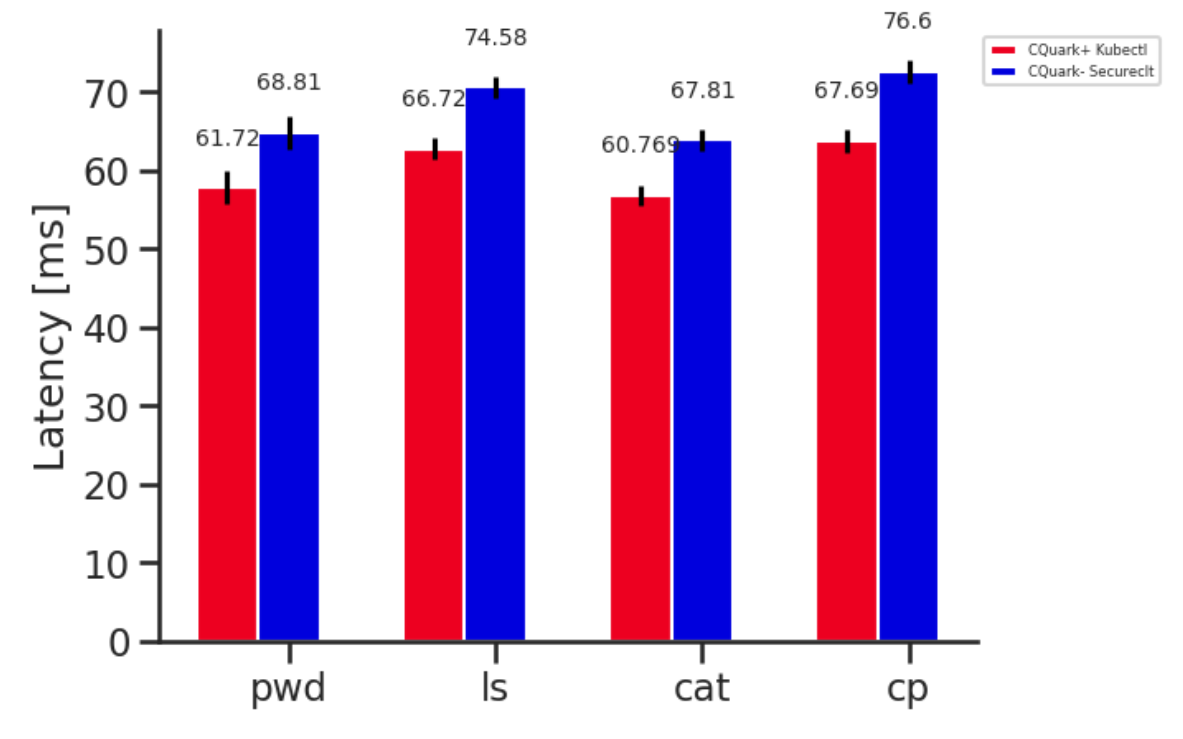
\includegraphics[width=0.8\textwidth]{images/speed_of_issuing_cmd_in_cquark_kubctl_securectl.PNG}
%     \caption[Benchmark result - Latency Comparison of issuing privileged instruction vs unprivileged instruction in confidential Quark]{A latency comparison test of issuing privileged instruction vs unprivileged instruction in confidential Quark.  The test included four frequently used Linux 
%     commands as samples, each being executed one thousand times.The results indicate that issuing privileged instructions is faster than issuing unprivileged instruction.
%     }
%     \label{fig:speed_of_issuing_cmd_in_cquark_kubctl_securectl}
% \end{figure}


% \begin{figure}[H]
%     \centering
%     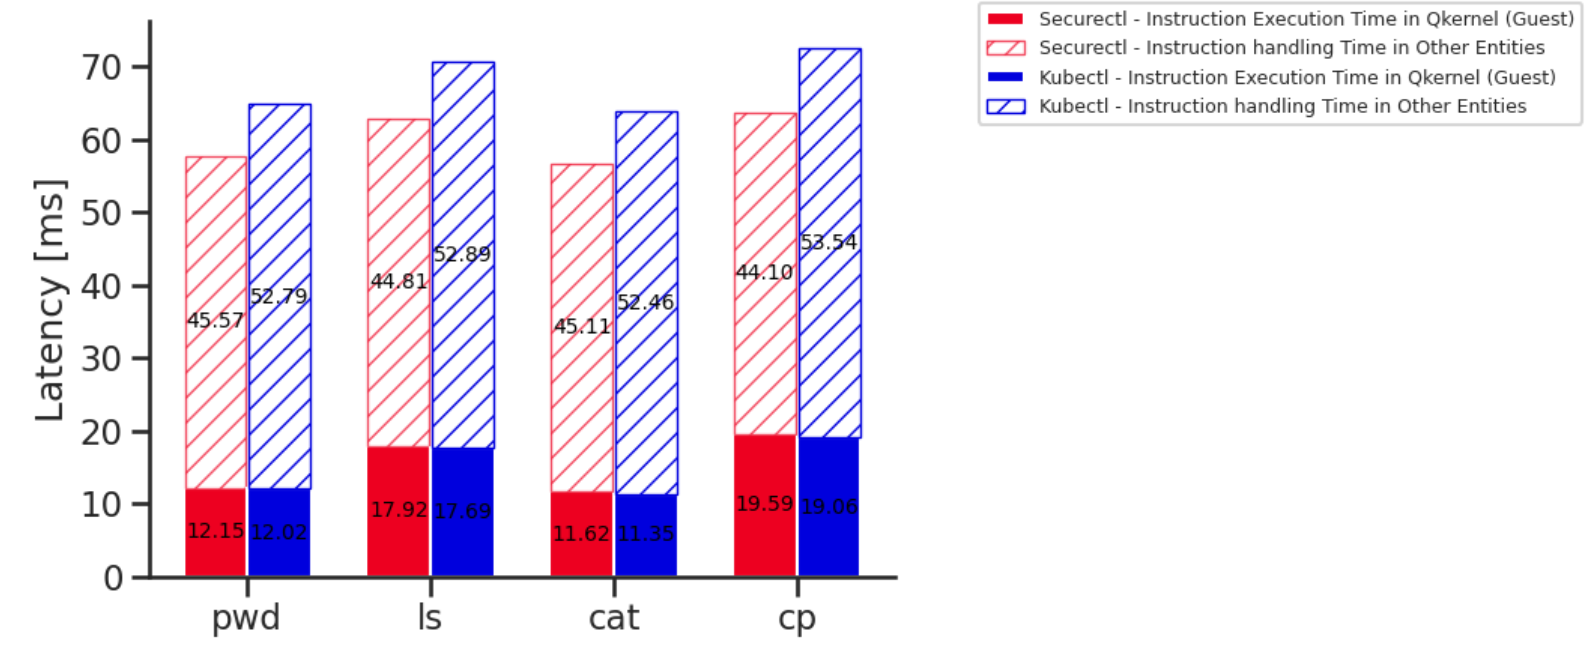
\includegraphics[width=0.8\textwidth]{images/timeshare_issuing_cmd_in_cquark_kubectl_securectl.PNG}
%     \caption[Benchmark result - The processing time for components during the privileged vs unprivileged instruction execution lifecycle]{Benchmark result evaluating the percentage of time spent by each component in processing instructions during the privileged versus unprivileged instruction 
%     execution lifecycle . Here the components refer to the tool the user employed to issue instructions, i.e., kubectl or securecli,  Kubernetes components for instructions transmission, like containerd, etc., and Qkernel for instruction execution.  Each bar in the 
%     figure represents the total execution time of an instruction whereby the color-filled section represents the time qkernel used for instruction execution, while the dashed-filled segment implies the time other components took for instruction issuing, transmission, and result handling.
%     }
%     \label{fig:timeshare_issuing_cmd_in_cquark_kubectl_securectl}
% \end{figure}



\subsection{Micro-benchmark – Latency Test for accessing binary-mapped memory region}\label{accesiing_binary_mapped_memory}

% //%or \small or \footnotesize etc.
% \begin{lstlisting}[language=C,frame=single,caption=Program for testing speed of accessing binary-mapped memory region Variant,label=code3,basicstyle=\tiny]
%     #define ARRAY_LEN (unsigned long)(1024*1024*100)    
%     char array[ARRAY_LEN] = {[ 0 ... (1) ] = 'a'} ;

%     int main {
%         struct timespec start, end;
%         clockid_t clk_id = CLOCK_MONOTONIC;  // CLOCK_REALTIME CLOCK_BOOTTIME CLOCK_PROCESS_CPUTIME_ID
%         struct timespec nanos;
%         clock_gettime(CLOCK_MONOTONIC, &nanos);
%         srand(nanos.tv_nsec); 
    
%         for(int i = 0; i < ARRAY_LEN; i++) {
%            index[i] = get_random();
     
%         }
     
%         clock_gettime(clk_id, &start);
%         for(int i = 0; i < ARRAY_LEN; i++) {
%            int current_idx = index[i];
%            //sequential read
%            // char a = array[i];
%            //sequential write
%            // array[i] = 'b';
%            //random read
%            // char a = array[current_idx];
%            //random write
%            // array[current_idx] = 'b';
%         }
%         clock_gettime(clk_id, &end);
     
%         unsigned long long  start_ns = to_ns(start);
%         unsigned long long  end_ns = to_ns(end);
%         printf("start %ju, end  %jun", start_ns, end_ns);

%         return 0;

%     }

 
% \end{lstlisting}

This section evaluates the speed of accessing binary-mapped memory regions at runtime. The benchmark utilizes a program~\cite*{benchamark_micro} containing a global initialized array and a for loop. The program can access the array within the for loop using four access modes: random read, random write, 
sequential read, and sequential write. We conduct the test in three binary data segment mapped memory sizes, i.e., 5MB, 10MB, and 100MB. For each case, the framework executes the program 30 times and calculates the average cost of accessing the array. Note that the size of the binary data segment 
mapped memory region is controlled by the size of the array. 








\begin{figure}[!htb] 
    \begin{subfigure}[b]{0.5\linewidth}
      \centering
      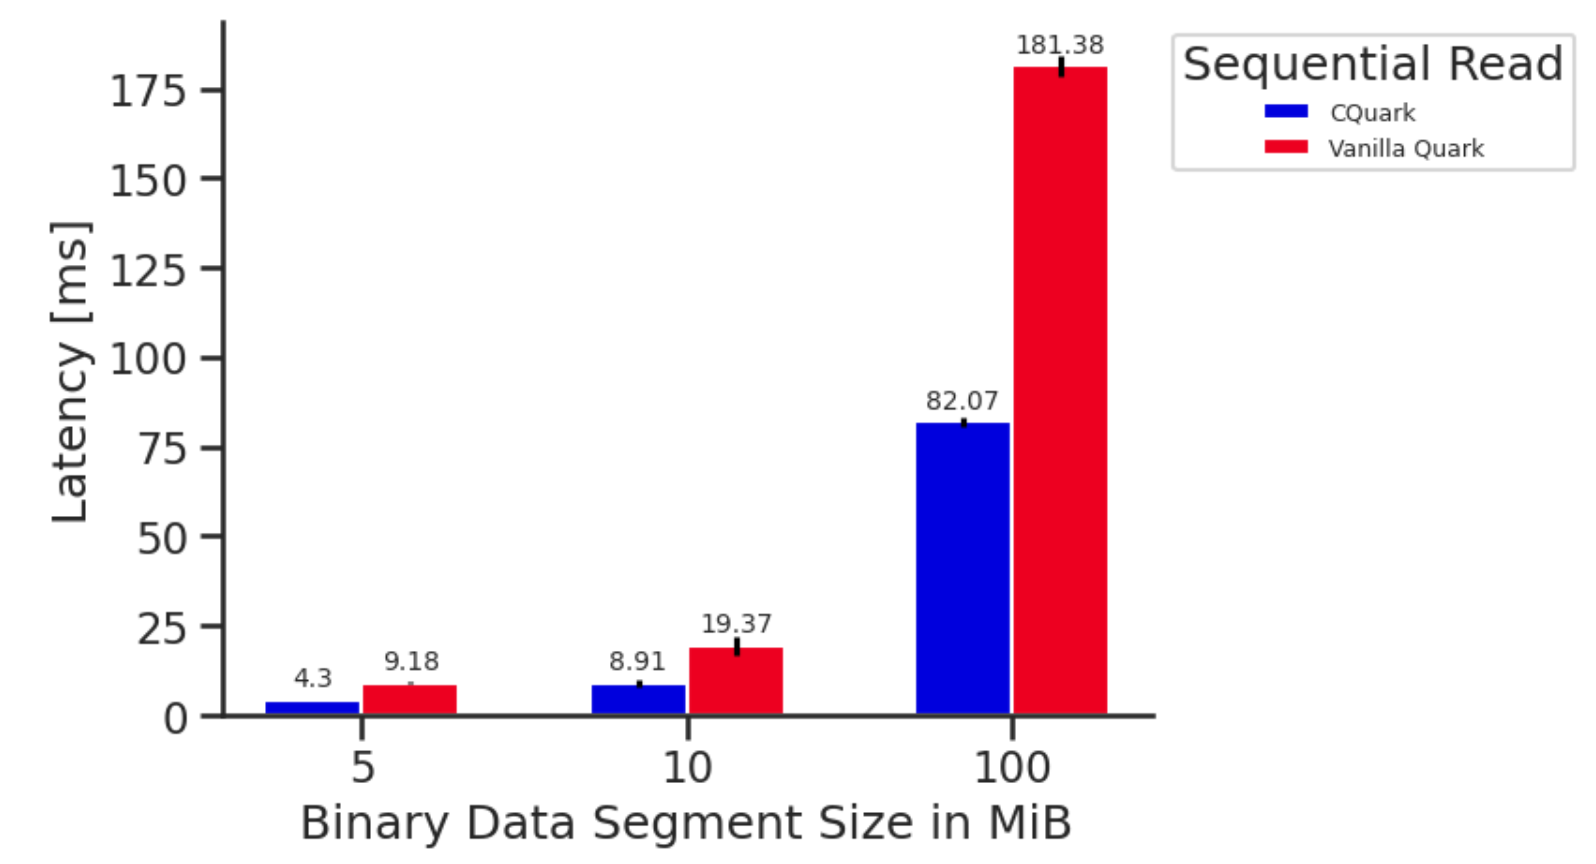
\includegraphics[width=0.9\linewidth]{images/Sequential_Read.PNG} 
      \caption{Sequential Read} 
      \label{fig7:a} 
      \vspace{4ex}
    \end{subfigure}%% 
    \begin{subfigure}[b]{0.5\linewidth}
      \centering
      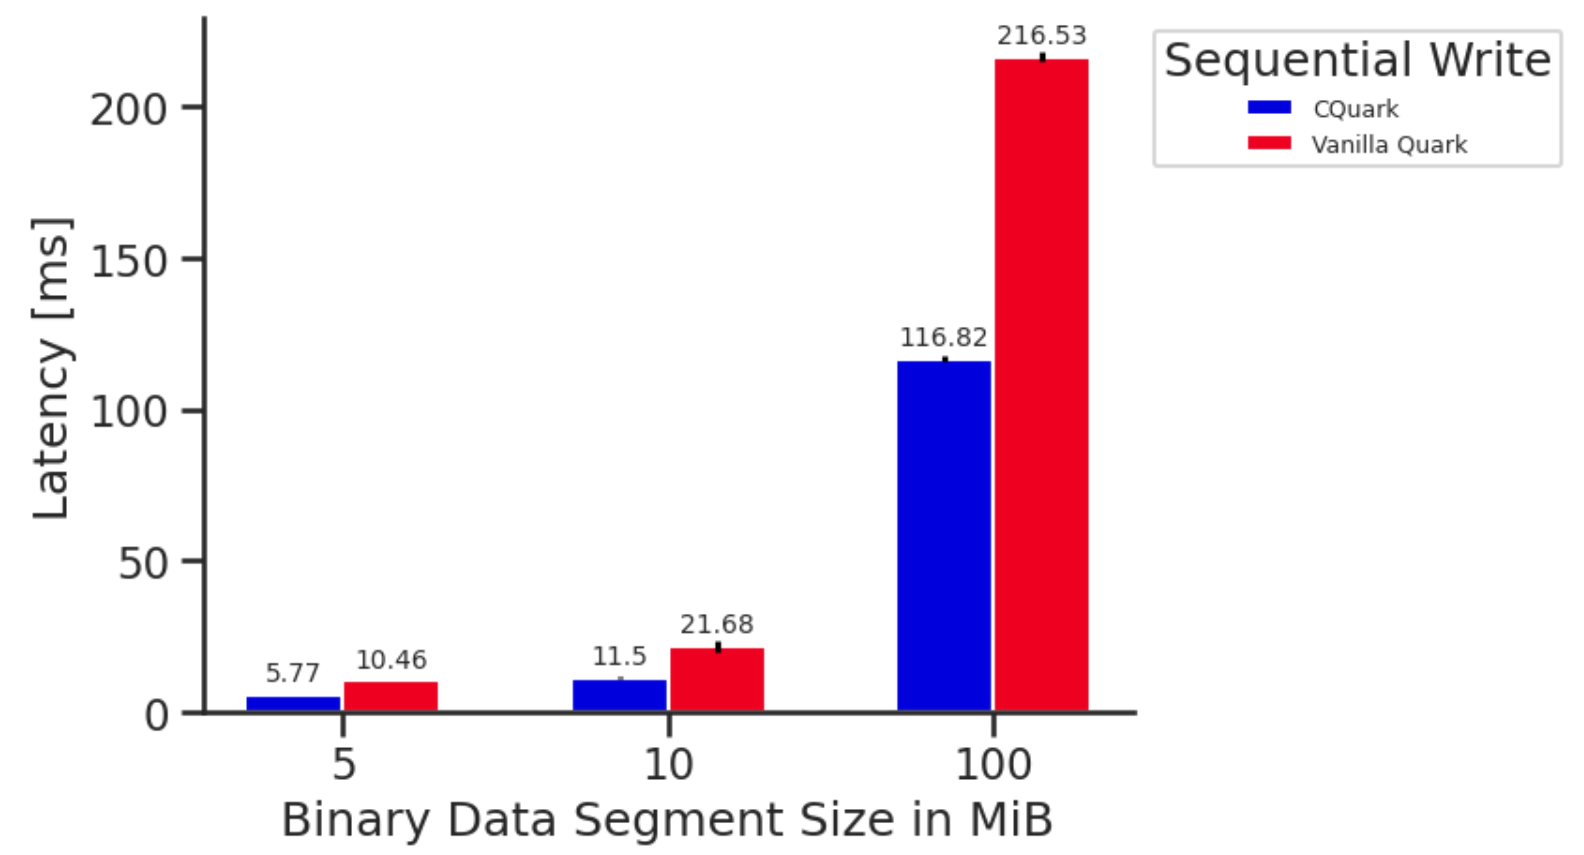
\includegraphics[width=0.9\linewidth]{images/Sequential_Write.PNG} 
      \caption{Sequential Write} 
      \label{fig7:b} 
      \vspace{4ex}
    \end{subfigure} 
    \begin{subfigure}[b]{0.5\linewidth}
      \centering
      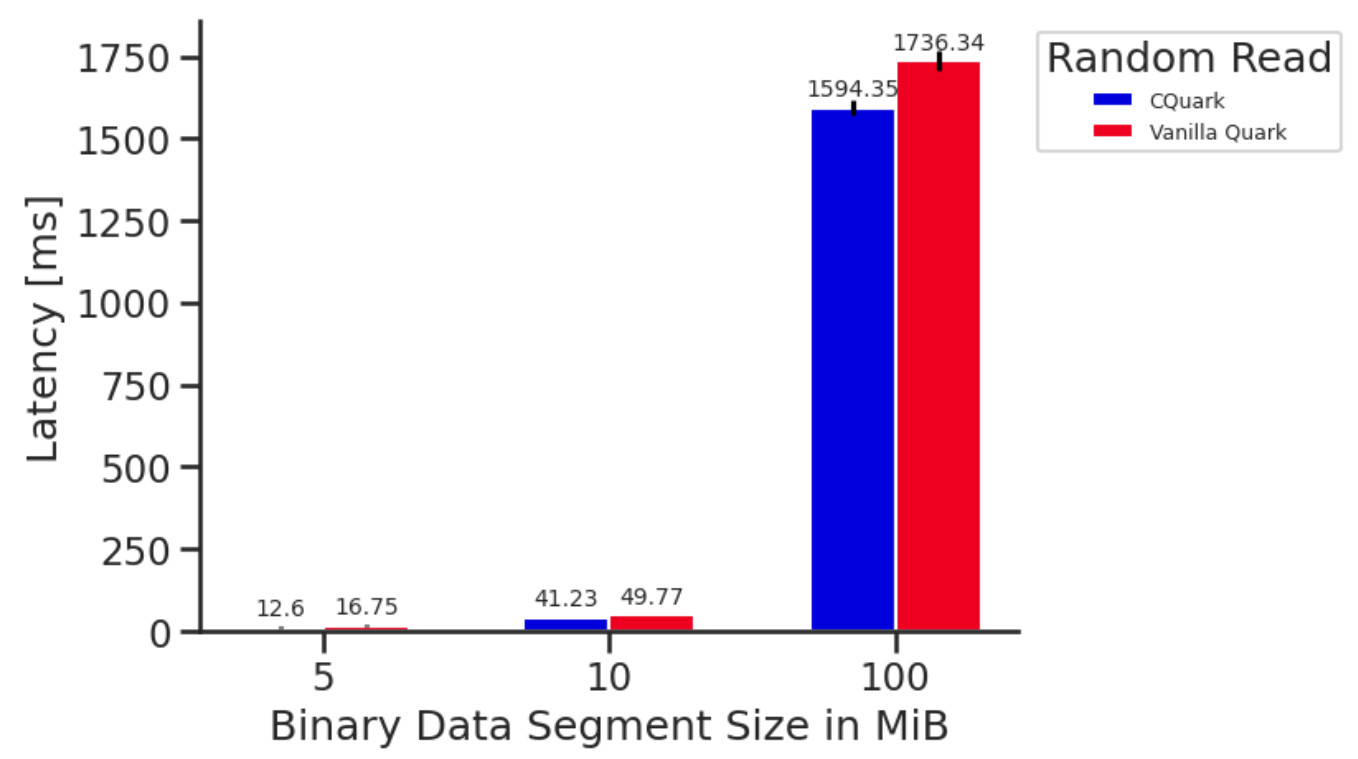
\includegraphics[width=0.9\linewidth]{images/Random_Read.PNG} 
      \caption{Random Read} 
      \label{fig7:c} 
    \end{subfigure}%%
    \begin{subfigure}[b]{0.5\linewidth}
      \centering
      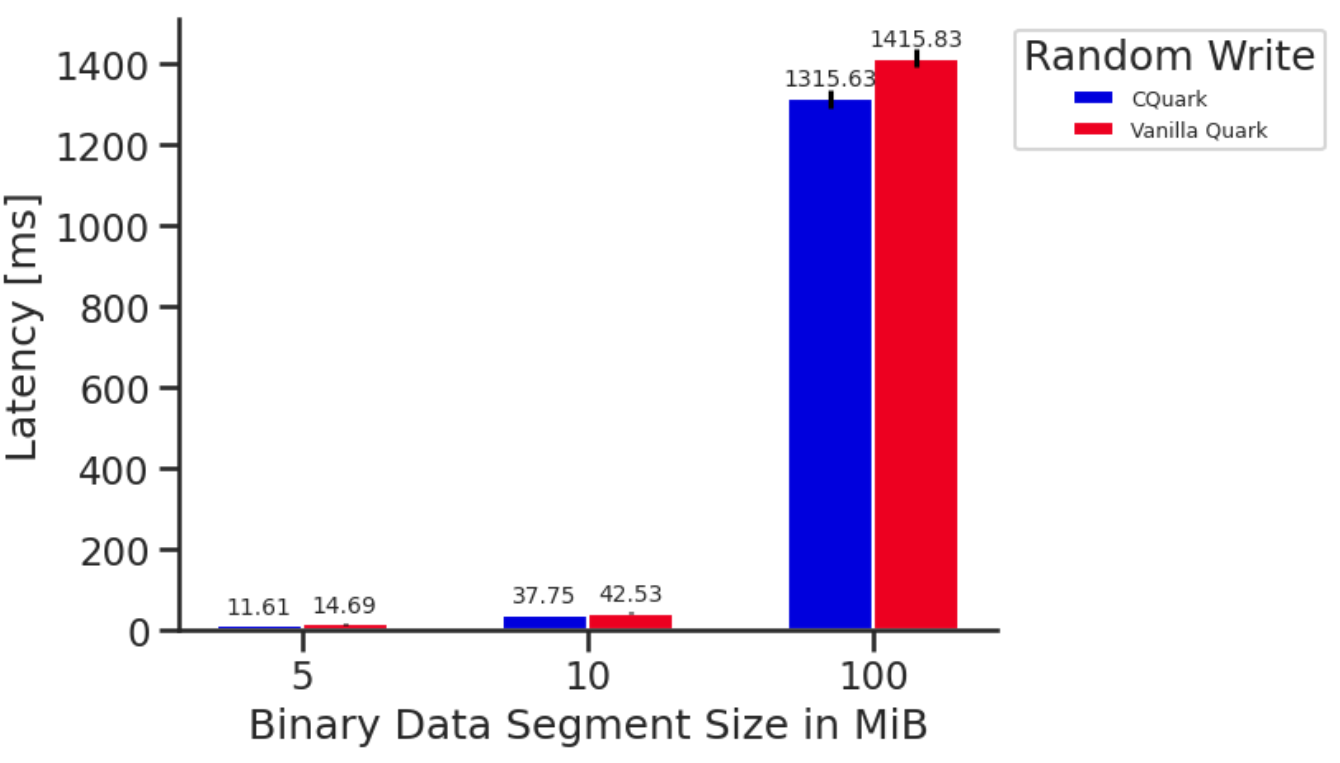
\includegraphics[width=0.9\linewidth]{images/Random_Write.PNG} 
      \caption{Random Write} 
      \label{fig7:d} 
    \end{subfigure} 
    \caption{Benchmark Result - Latency Test for accessing binary-mapped memory region}
    \label{fig7} 
\end{figure}



The results shown in Figures~\ref{fig7:a} and~\ref{fig7:b} indicate that the sequential access in the confidential Quark is 1.86 times faster than in the vanilla Quark. The reason is that confidential Quark preloads the binary into the guest memory before the program launches, thus avoiding page fault handling at 
runtime. For the same reason, random reads and writes in confidential Quark are 1.08 times faster than in vanilla Quark (Figure ~\ref{fig7:c} and Figure ~\ref{fig7:d}).


\subsection{Micro-benchmark – Latency Test for Application Startup}\label{micro_app_start_up}

This section evaluates the latency overhead that the shield imposes on application startup. As described in Chapter~\ref{sec:implementation}, two factors may affect the application startup time: the number of file type secrets and the data size measured by the Software Measurement Manager. Therefore, 
the following three tests are performed in this section. First, we establish a baseline by setting the number of file type secrets to zero and running the hello world program. In this case, the enclave only obtains the enclave policy from the secret manager. In Experiment 2, we increase the number of 
file type secrets to observe the change in program startup time. Experiment 3 examines how increasing the binary size affects the program startup time.

\begin{lstlisting}[language=C,frame=single,caption=Hello World Program Variant,label=code2]
#define ARRAY_LEN (unsigned long)(1024*1024*100)    
char array[ARRAY_LEN] = {[ 0 ... (1) ] = 'a'} ;
int main() {     
    printf("Hello, World!\n");
    return 0;
}
\end{lstlisting}

    
We extend the test framework~\cite*{benchamark_framework} to start and terminate the application iteratively. It measures the mean and variance of the program startup time and evaluates the overhead imposed by the components in the shield. These components include the remote attestation and 
provisioning agent,  secret injector,  hardware evidence driver, and software measurement manager. Additionally, we use the statically connected hello world program from Listing~\ref{code2} as the test workload, which contains a global initialization array to regulate the binary data segment size. 
The framework will run the application 100 times. For the methodology for measuring the overhead introduced by the shield component, we refer the user to Section~\ref{Hardware_and_Software_Setup}.

\begin{figure}[!htb]
    \centering
    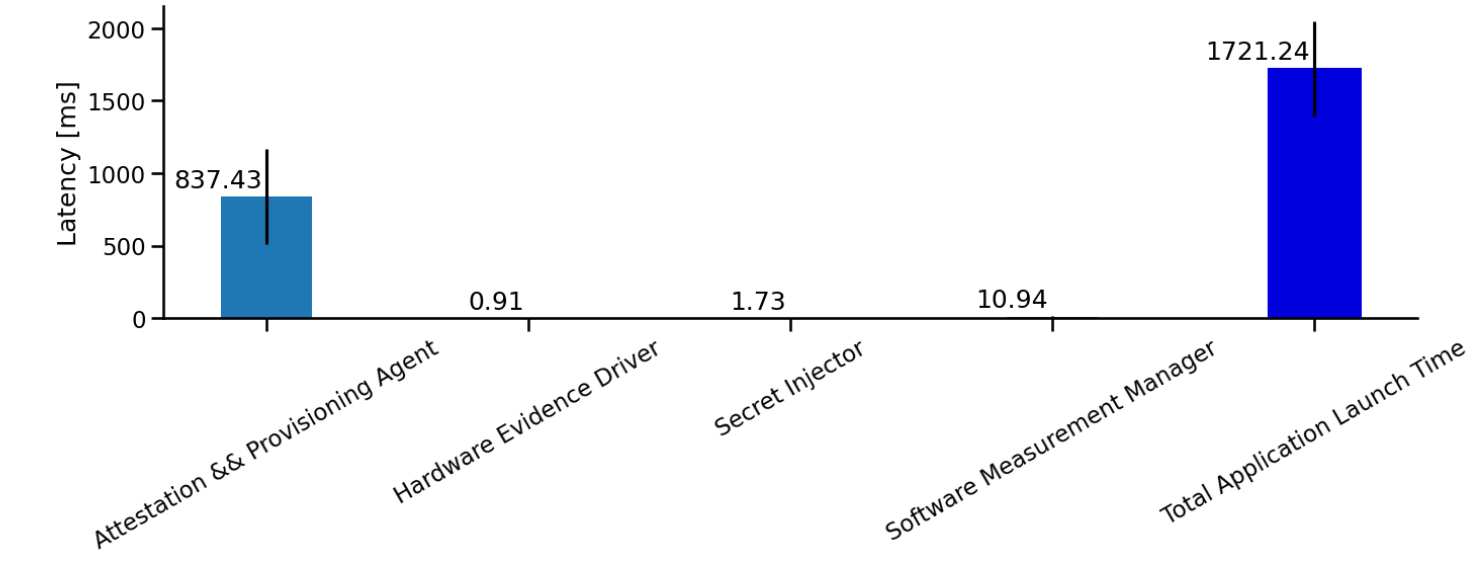
\includegraphics[width=0.7\textwidth]{images/application_start_microtest_baseline_time_overhead_each_cmp.PNG}
    \caption[Baseline: latency overhead introduced by shielding layer]{Baseline: latency overhead introduced by shielding layer}
    \label{fig:application_start_microtest_baseline_time_overhead_each_cmp}
\end{figure}


\begin{table}[!htb]
    \centering
    \footnotesize
    \caption{Software measurement manager measured data during application startup\strut}
    \begin{tabularx}{1\textwidth}{@{} l L L L L L L@{}}
    \toprule
        Matrics    & ELF &  Shared Lib   & Qkernel Config File    & Public Key of Secret Manager  & Total\\
    \midrule

        \vn{Measurement}     &  1.447 MiB    &   0 MiB  &   534 Byte      &2017 Byte  & 1.449 MiB\\
    \bottomrule
    \end{tabularx}
    \label{table: Measurement_For_Hello_world}
\end{table}
\todo{fix the table}

The baseline results in Figure~\ref{fig:application_start_microtest_baseline_time_overhead_each_cmp} show that the shielding layer doubled the program startup time. Notably, the remote attestation and provisioning agent contributed the most to the latency overhead, which is expected since it must establish a TLS connection with the relying party, complete the 
remote attestation process, and retrieve the secrets. The Secret Injector, Hardware Evidence Driver, introduces a latency overhead of 0.90 ms and 1.73 ms. However, this latency is negligible compared to the overhead caused by the attestation agent (837 ms). In addition, the data in 
Table~\ref{table: Measurement_For_Hello_world} indicates that the Software Measurement Manager measured approximately 1.449 MiB of data during program startup, resulting in an overhead of only 10 milliseconds. 

\begin{figure}[!htb]
    \centering
    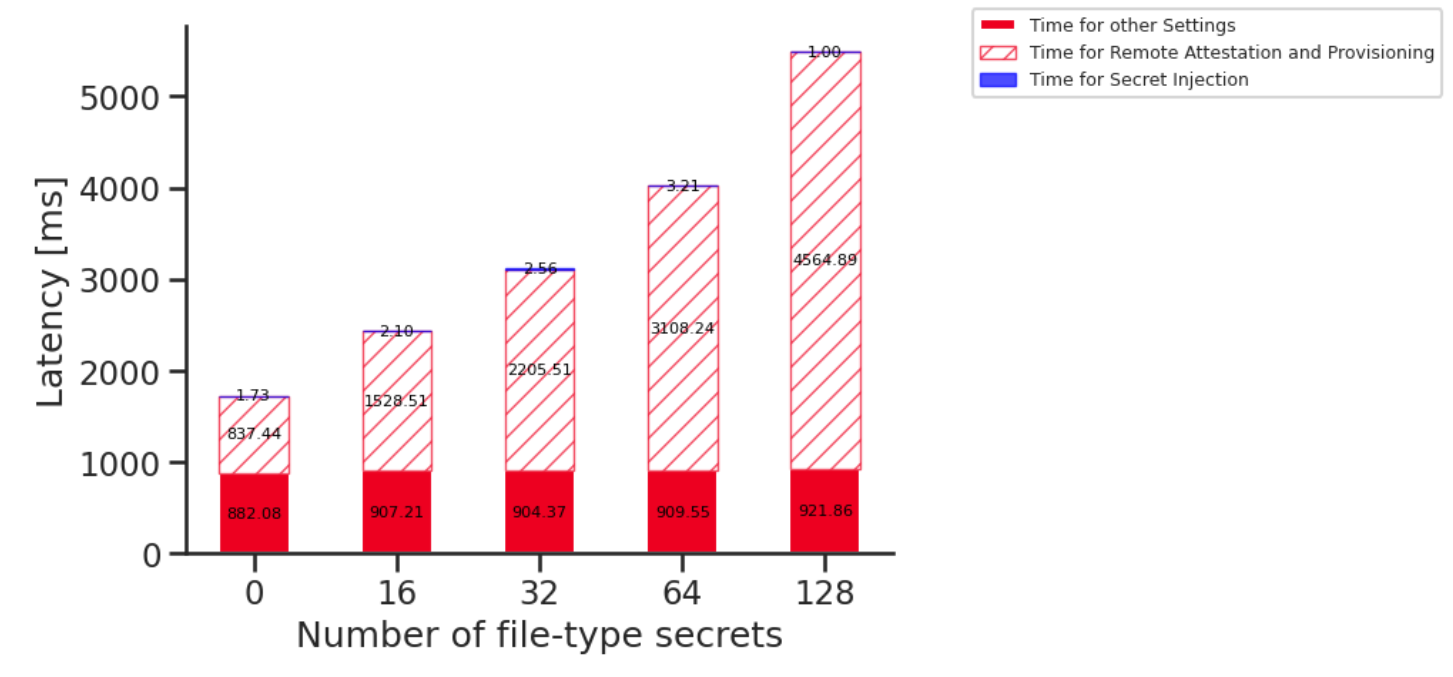
\includegraphics[width=0.8\textwidth]{images/startup_time_change_as_file_type_secret_increasing.PNG}
    \caption[Distribution of the time consumed by attestation \&\& provisioning agent, secret injector and others in the application startup]{Distribution of the time consumed by attestation \&\& provisioning agent, secret injector and others in the application startup}
    \label{fig:startup_time_change_as_file_type_secret_increasing}
\end{figure}

Figure~\ref{fig:startup_time_change_as_file_type_secret_increasing} shows how the latency overhead of the remote attestation and provisioning agent changes as the number of file-type secrets increases. The overhead from the remote authentication and provisioning agent is proportional to the 
number of file type secrets because it must perform one HTTP + TLS operation for each file. When the number of file-type secrets reaches 128, the overhead associated with the agent becomes astounding, reaching 4500 ms, accounting for over 70\% of the total program startup time.
\begin{figure}[!htb]
    \centering
    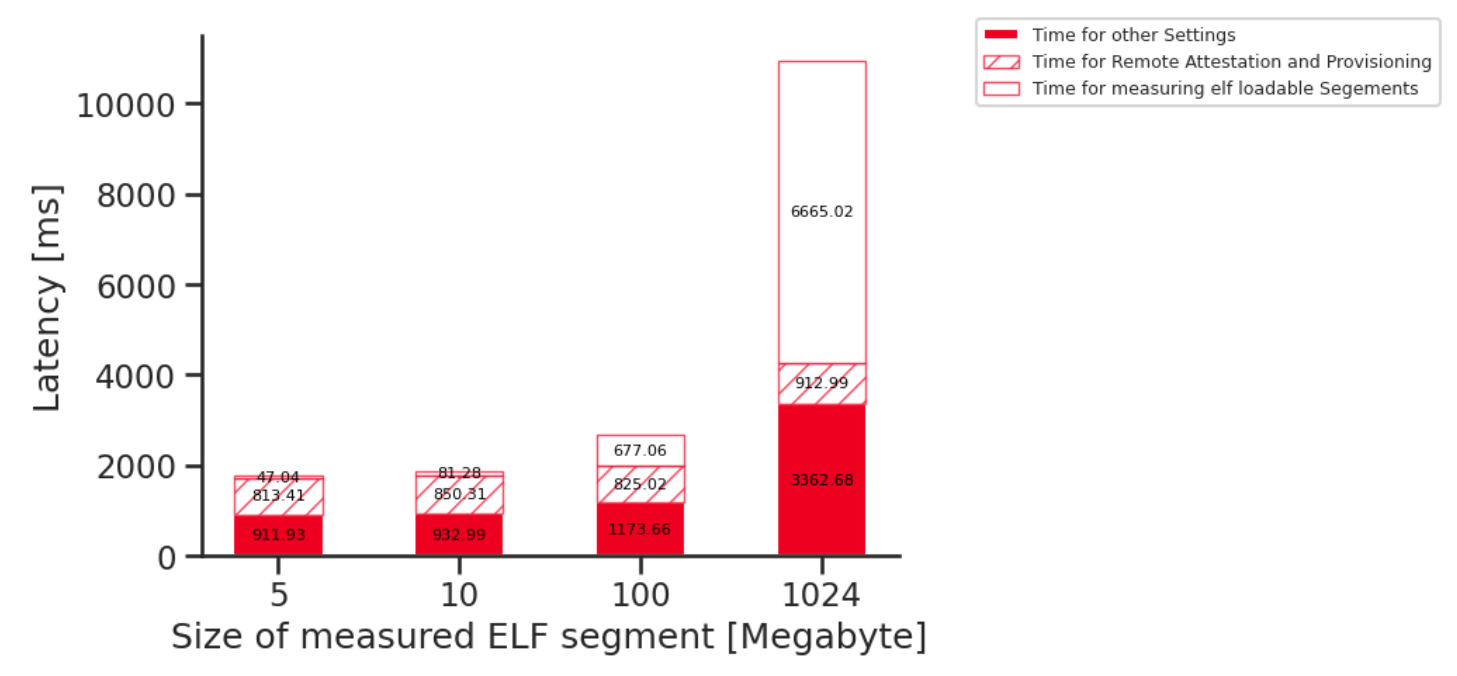
\includegraphics[width=0.8\textwidth]{images/startup_time_change_as_elf_size_increasing.PNG}
    \caption[Distribution of the time consumed by software measurement manager and others in the Application Startup]{Distribution of the time consumed by software measurement manager and others in the Application Startup}
    \label{fig:startup_time_change_as_elf_size_increasing}
\end{figure}


Figure~\ref{fig:startup_time_change_as_elf_size_increasing} shows that the latency overhead of the software measurement manager is proportional to the size of the binary. Besides, when the measured data is less than or equal to 100MB, the latency overhead of the software measurer is lower than the 
overhead introduced by the remote attestation and provisioning agent.






% \begin{figure}[H]
%     \centering
%     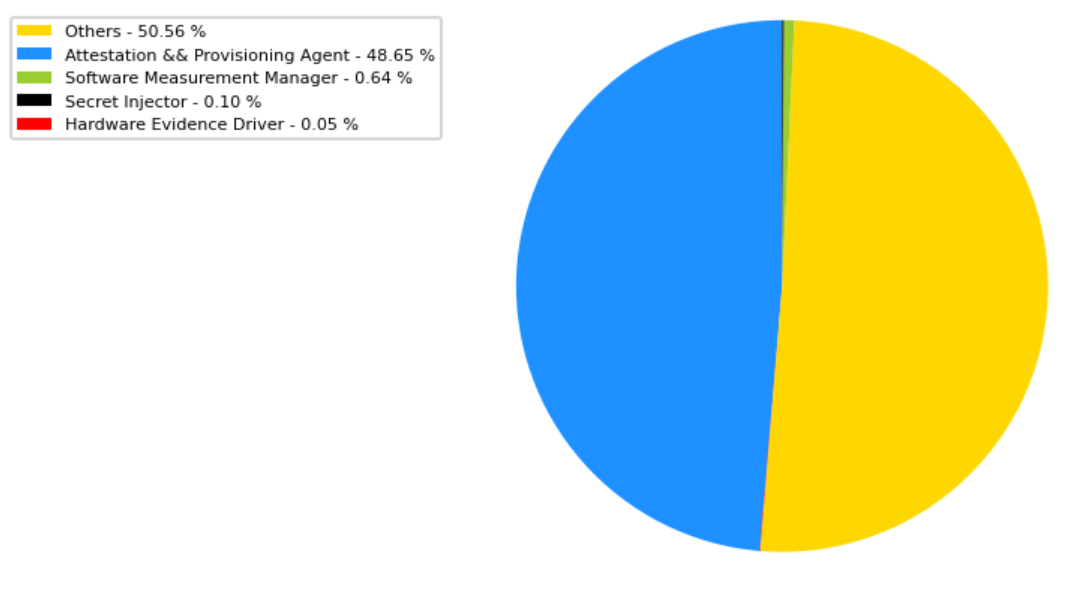
\includegraphics[width=0.8\textwidth]{images/application_start_microtest_baseline_time_distribution.PNG}
%     \caption[Time  Distribution of the application startup ]{Distribution of the time consumed by different components in the application startup}
%     \label{fig:application_start_microtest_baseline_time_distribution}
% \end{figure}




% \begin{figure}[H]
%     \centering
%     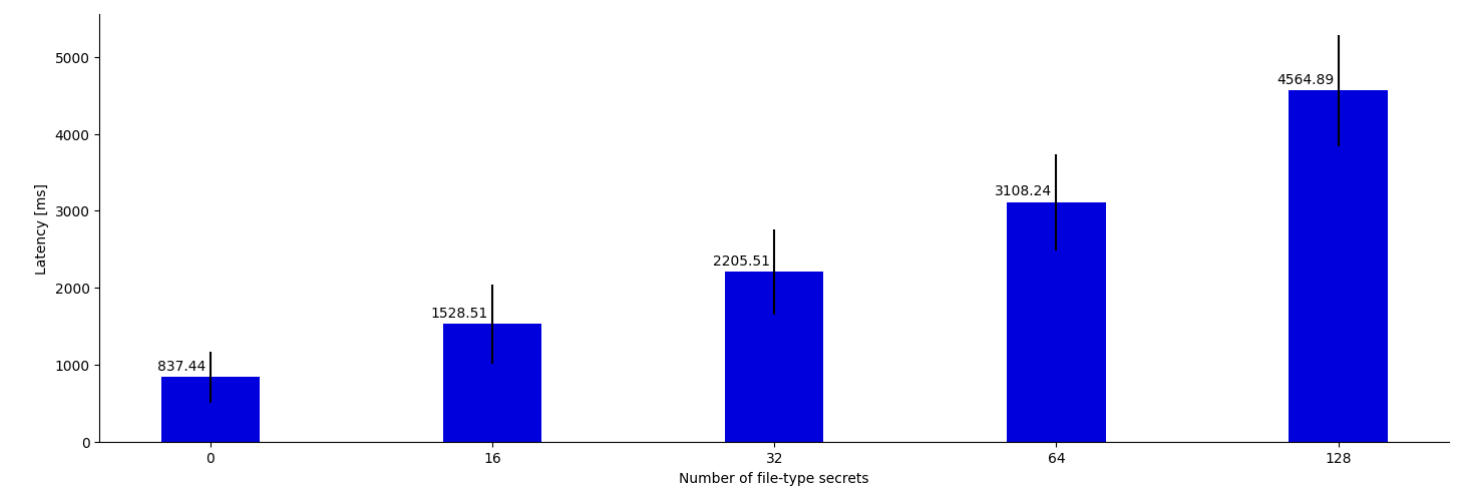
\includegraphics[width=0.8\textwidth]{images/overhead_attestation_agent_as_file_num_increasing.PNG}
%     \caption[Benchmark result: Latency Overhead from Attestation \&\& Provisioning Agent as the number of file-based secrets increases]{Benchmark result: Latency Overhead from Attestation \&\& Provisioning Agent as the number of file-based secrets increases}
%     \label{fig:overhead_attestation_agent_as_file_num_increasing}
% \end{figure}


% , which reveal the evolution of the overhead introduced by the remote attestation and provisioning agent, and 
% secret injector, as the number of file-type secrets grows.





% \begin{figure}[H]
%     \centering
%     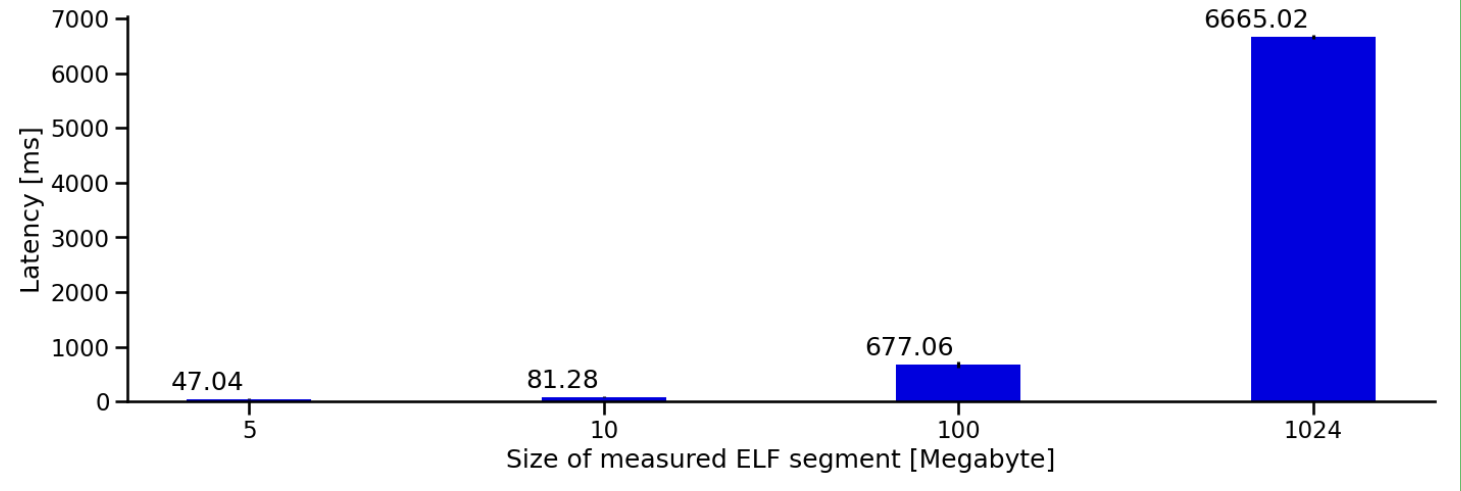
\includegraphics[width=0.8\textwidth]{images/overhead_software_measurement_manager_as_elf_size_increasing.PNG}
%     \caption[Benchmark result: Latency Overhead from Software Measurement Manager as the measured Data Size increases]{Benchmark result: Latency Overhead from Software Measurement Manager as the measured Data Size increases}
%     \label{fig:overhead_software_measurement_manager_as_elf_size_increasing}
% \end{figure}




\subsection{Macro-Benchmark– Application Life Cycle Performance Benchmark}\label{macri_app_start_up}

This section evaluates the performance of running real-world applications in confidential and vanilla Quark. We chose Nginx~\cite*{nginx} and Redis~\cite*{redis} as test subjects and compared their startup time, exit time, and runtime throughput. At program runtime, we use the Apache HTTP Server 
Benchmarking Tool (AB)~\cite*{ab} and Redis-benchmark~\cite*{Redis_benchmark} to generate workloads for Nginx and Redis, respectively.

Regarding the benchmarking methodology, we extended the testing framework~\cite*{benchamark_framework} to repeatedly launch the target application 100 times, record its startup and exit times, and the results of AB and Redis-benchmark. Redis benchmark and AB
 are set to issue 1,000,000 requests using 50 concurrent clients to Redis and Nginx, respectively. In addition, the file size requested by ab from Nginx is 181 bytes. In addition, AB requests a file size of 181 bytes from Nginx. Both applications fetch enclave policy from the secret manager only.


 \begin{figure}[!htb]
  \centering
  \includegraphics[width=0.5\textwidth]{images/reds_nginx_startup_comp.PNG}
  \caption[Redis \&\& Nginx Startup Time in Cquark vs vanilla Quark]{Redis \&\& Nginx Startup Time in confidential vs vanilla Quark}
  \label{fig:reds_nginx_startup_comp}
\end{figure}


\begin{figure}[!htb]
  \centering
  \includegraphics[width=0.8\textwidth]{images/time_disribution_startup_redis_nginx.PNG}
  \caption[Redis \&\& Nginx  Startup Time in Cquark vs vanilla Quark]{Redis \&\& Nginx  Startup Time in Cquark vs vanilla Quark}
  \label{fig:time_disribution_startup_redis_nginx}
\end{figure}
\todo{fix naming issue kbs client to attestation agent}


\begin{table}[!htb]
  \centering
  \scriptsize

  \begin{tabularx}{1\textwidth}{@{} l L L L L L L@{}}
  \toprule
      Matrics    & ELF &  Shared Library   &Qkernel Config File    & Public Key of Secret Manager  & Total Measurement\\
  \midrule

      \vn{Measurement for Redis}     &  3.64 MiB   &   12.61 MiB  &   534 Byte      &2017 Byte   & 16.25 MiB\\
      \vn{Measurement for Nginx}     &  5.5 MiB    &   61.64 MiB  &   534 Byte      &2017 Byte   & 67.14 MiB\\
  \bottomrule
  \end{tabularx}
  \caption{Software Measurement Manager measured Data during Application Startup\strut}
  \label{table:Measurement_For_Nginx_Redis}
\end{table}

The results shown in Figure~\ref{fig:reds_nginx_startup_comp} indicate that confidential Quark takes about twice as long as vanilla Quark to complete the application setup. This result is reasonable because the confidential Quark must perform additional operations such as remote attestation and 
measuring data loaded from the host. When comparing the startup times of Nginx and Redis in Confidential Quark, we observe that Nginx takes about 324 ms longer than Redis. From Fig~\ref{fig:time_disribution_startup_redis_nginx}, we find that the difference mainly comes from the latency overhead 
difference of the software measurement manager and the remote attestation and provisioning agent, i.e., 424 ms and 65 ms, respectively. Since both applications retrieve the same number of secrets from the secret manager, we speculate that the difference in remote attestation and provisioning 
agent's overhead comes from network jitter or measurement errors. In addition, Table~\ref{table:Measurement_For_Nginx_Redis} shows that the software measurement manager measured 67.14 and 16.25 Mb in Nginx and Redis, respectively. Because the software measurement manager has to measure more data in 
Nginx, its latency overhead is larger in Nginx. 

\begin{figure}[!htb]
  \centering
  \includegraphics[width=0.5\textwidth]{images/reds_nginx_exit_comp.PNG}
  \caption[Redis \&\& Nginx Exit Time in Cquark vs vanilla Quark]{Redis \&\& Nginx Exit Time in Cquark vs vanilla Quark}
  \label{fig:reds_nginx_exit_comp}
\end{figure}
Figure~\ref{fig:reds_nginx_exit_comp} shows that the exit time for Redis and Nginx is around 2529 milliseconds in both confidential Quark and vanilla Quark, as confidential Quark does not modify the critical path for program exit.
\begin{figure}[!htb]
  \centering
  \includegraphics[width=1\textwidth]{images/redis_throughput.PNG}
  \caption[Redis Throughout Test]{Redis Throughout Test Result}
  \label{fig:redis_throughput}
\end{figure}


\begin{figure}[!htb]
  \centering
  \includegraphics[width=0.5\textwidth]{images/nginx_throughput.PNG}
  \caption[Nginx Throughout Test]{Nginx Throughout Test Result}
  \label{fig:nginx_throughput}
\end{figure}

The throughput test results for Redis and Nginx are shown in Figure~\ref{fig:redis_throughput} and Figure~\ref{fig:redis_throughput}. Our analysis shows that executing Redis and Nginx in confidential Quark leads to about 22\% and 10\% performance degradation, respectively. 
The possible reason for this impact is the overhead introduced by intercepting guest system calls.


\subsection{Trust Computing Base}\label{tcb}

This section evaluates the TCB overhead introduced by our implementation and compares the TCB sizes of confidential Quark and Kata containers~\cite*{Kata-Containers}. To this end, we compare the lines of code and the size of the guest kernel binary for confidential and vanilla Quark. Note that the 
guest kernel binary comprises the code from 3 components, Qkernel, Qlib, and the shielding layer. In comparing the TCB sizes of confidential Quark and Kata containers, we use the binary sizes of the guest assets as a reference. The assets for confidential Quark are the Qkernl binary, while the 
assets for the Kata container include the Kata agent~\cite*{kata_agent}, OVMF~\cite*{ovmf}, and the Linux kernel. To ensure fairness, we use the strip utility~\cite*{strip} to remove unused symbols from the binaries.

\begin{table}[htbp]
  \centering
\begin{tabular}{lrrrcrrr}\toprule
  \hline
  \multicolumn{3}{c}{Vanilla Quark}&&\multicolumn{3}{c}{Confidential Quark}\\
  \cline{1-3}\cline{5-7}
  $Component$ & $LoC$ & $Size$$^{3}$ && $Component$ & $LoC$ & $Size$$^{3}$\\
\midrule
   Qkernel &32487 & -&& Qkernel&32487&-\\
   Qlib &85128  & -&&Qlib&  86609 &-\\
   Shield  & 0 & - && Shield&2805&-\\

   \midrule
    Total  & 117615& 3.1MiB&& & 121901 &  4.6 MiB\\
    \bottomrule
\end{tabular}

\caption{Comparison of the LoC and compiled size of vanilla quark and confidential quark\strut}
\label{table:tcb_size_quark_vs_cquark}
\end{table}


Table~\ref{table:tcb_size_quark_vs_cquark}  summarizes the TCB overhead required to implement secrecy in Secrecy Quark. Vanilla Quark's guest kernel has 117615 lines of code and generates a statically linked binary of 3.10 MB. In Secrecy Quark, our implementation adds 4286 lines of code to the guest kernel binary, bringing the total 
number of lines of code to 121981, and the binary reaches 4.6 MB. Overall, our implementation increases the size of the guest binary by a factor of 1.48 compared to vanilla Quark.
\begin{table}[htbp]
  \centering
\begin{tabular}{lrrcrr}\toprule
  \hline
  \multicolumn{2}{c}{Kata Container}&&\multicolumn{2}{c}{Confidential Quark}\\
  \cline{1-2}\cline{4-5}
  $Component$  & $Size$$^{3}$ && $Component$  & $Size$$^{3}$\\
\midrule
   Guest Kernel &47.16 MiB && Guest kernel &4.6 MiB\\
   OVMF   & 4 MiB && &   &\\
   Kata agent  & 22.65MiB  && &&\\

   \midrule
      & 73.81 MB&& &   4.6 MiB\\
    \bottomrule
\end{tabular}

\caption{TCB size comparison between kata container vs. confidential quark in terms of binary size of guest assets \strut}
\label{table:tcb_size_quark_vs_kata}
\end{table}

Table~\ref{table:tcb_size_quark_vs_kata} compares the size of TCBs in the kata container and the confidential Quark. In the Kata container, the binary sizes of the Kata agent, OVMF, and guest kernel are 22.65 MB, 4.0 MB, and 47.16 MB, respectively. The total TCB size is 73.81 MB, about 16 times that of the confidential 
Quark.

\section{Summary}
I conducted qualitative and quantitative analyses in this chapter to evaluate my work. In the qualitative analysis, I identified potential security vulnerabilities in vanilla Quark and explained how my work mitigates these vulnerabilities. 
Regarding the quantitative analysis, I developed a testing framework to characterize the performance of CQuark. The results showed that confidential Quark engenders significant overhead compared to vanilla Quark. 
This overhead is visible in longer program creation times, reduced runtime program throughput, reduced speed of issuing instructions to the program, increased trusted computing base (TCB) size, etc.




% \begin{table}[htp]
%     \caption{Software measurement manager measured data during application startup}
%     \begin{tabularx}{\textwidth}{*{2}{p{0.5\textwidth}}}\toprule
%                                  & ELF &  Shared Library   & Process Spec  & Stack   & Guest Kernel Args  & Total Measurement \\ \midrul
%     Measurement For Hello world  &  1.4468 MiB    &   0 MiB  &   3819 Byte   & 305 Byte   &5865 Byte  & 1.457 MiB \\\addlinespace
%     \bottomrule
%     \end{tabular}
%     \label{table: Measurement_For_Hello_world}
% \end{table}


% \begin{table}[!ht]
%     \sffamily
%     \caption{Terminologies in SQL \& corresponding in MongoDB}
%     \label{tab:my_label}
%     \centering
%     \begin{tabularx}{\textwidth}{*{2}{p{0.5\textwidth}}}
%     \toprule
%                                  & ELF &  Shared Library   & Process Spec  & Stack   & Guest Kernel Args  & Total Measurement \\ \midrule
%     Measurement For Hello world  &  1.4468 MiB    &   0 MiB  &   3819 Byte   & 305 Byte   &5865 Byte  & 1.457 MiB \\\addlinespace
%     \dots & \dots \\
%     \bottomrule
%     \end{tabularx}
%     \end{table}




\cleardoublepage

%%% Local Variables:
%%% TeX-master: "diplom"
%%% End:
